%! Author = saili
%! Date = 2019/8/23/0023

% Preamble
\documentclass{article}
%! Author = saili
%! Date = 2019/8/26/0026
% Packages
\usepackage{amsmath}%提供数学公式支持

\usepackage{graphics}%用于添加图片
\usepackage{graphicx}%加强插图命令
\usepackage{subfigure}%用于添加子图
\usepackage{wrapfig}%提供图片环绕风格支持
\graphicspath{{./}{./contents/}{./contents/fig/}}%设置图片可能存在的路径
\newcommand{\figpath}[1]{contents/fig/#1}

\usepackage{fontspec}%用于配置字体
\usepackage[table]{xcolor}%用于各种颜色环境
\usepackage{enumitem}%用于定制list和enum
\usepackage{float}%用于控制Float环境,添加H参数(强制放在Here)
\usepackage[colorlinks,linkcolor=airforceblue,urlcolor=blue,anchorcolor=blue,citecolor=green]{hyperref}%用于超链接,另外添加该包目录会自动添加引用。

\usepackage[most]{tcolorbox}%用于添加各种边框支持
\usepackage[cache=true,outputdir=./out]{minted}%如果不保留临时文件就设置cache=false,如果输出设置了其他目录那么outputdir参数也有手动指定,否则会报错。
\tcbuselibrary{minted}%加载tcolorbox的代码风格

\usepackage[a4paper,left=3cm,right=3cm,top=3cm,bottom=3cm]{geometry}%用于控制版式
\usepackage{appendix}%用于控制附加文件
\usepackage{ifthen}

\usepackage{pdfpages}%用于支持插入其他pdf页
\usepackage{booktabs}%目前用于给表格添加 \toprule \midrule 等命令
\usepackage{marginnote} %用于边注
\usepackage[pagestyles,toctitles]{titlesec} %用于标题格式DIY
% \usepackage{fancyhdr}%用于排版页眉页脚
\usepackage{ragged2e} % 用于对齐
%! Author = saili
%! Date = 2019/8/23/0023

\definecolor{todored}{rgb}{0.58,0,0}
\definecolor{hlyellow}{rgb}{0.9765,0.7922,0.1412}
\definecolor{hlgree}{rgb}{0.18,0.8,0.44}
\definecolor{hlblue}{rgb}{0.20,0.59,0.85}
\definecolor{test}{RGB}{106, 176, 76}

% tcolorbox系列
\definecolor{boxtitleback}{rgb}{0.17,0.24,0.31}
\definecolor{boxback}{RGB}{245,246,250}

\definecolor{codeback}{rgb}{0.9647,0.9725,0.9804}
%! Author = saili
%! Date = 2019/8/23/0023


\newcommand{\sitem}{\subitem $-$}
%\newcommand{\sitem}{{\setlength{\itemindent}{5pt} \subitem $-$ }}

%! Author = saili
%! Date = 2019/8/26/0026
\usepackage{layout} %用于生成布局图片
\usepackage{multirow} %用于表格环境多行多列的支持
\usepackage{pdfpages} %用于插入pdf页
\usepackage{rotating} %提供旋转、横置页面的方法
\usepackage{adjustbox} %用于调整盒子
\usepackage{ulem} %用于好看的下划线、波浪线等修饰

\usepackage{supertabular} %用于提供长表格支持
\usepackage{longtable}% 用于提供长表格支持

\usepackage{fixltx2e} %用于文本环境的下标
\usepackage{nameref} % 用于在引用时使用名字
\definecolor{airforceblue}{rgb}{0.36, 0.54, 0.66}
\newcommand{\Ref}[1]{\textcolor{airforceblue}{\ref{#1}:\nameref{#1}}}
\newlength\tablewidth
\newtcblisting{texcode}{
    arc=0mm,drop shadow,
    externalize listing=example_listing,
    listing engine=minted,
    minted style=colorful,
    minted language=tex,
    minted options={fontsize=\small,breaklines,autogobble,numbersep=0mm},
    colback=codeback,
    colframe=codeback,
    listing only,
    left=0mm,enhanced,
}

\newtcblisting{texbreakcode}{breakable,
    arc=0mm,drop shadow,
    externalize listing=example_listing,
    listing engine=minted,
    minted style=colorful,
    minted language=tex,
    minted options={fontsize=\small,breaklines,autogobble,numbersep=0mm},
    colback=codeback,
    colframe=codeback,
    listing only,
    left=0mm,enhanced,
}

\newtcblisting{texbreakshow}{breakable,
    arc=1mm,drop shadow,
    title=Code effects,
    coltitle=langtitle,
    colbacktitle=langbacktitle,
    colframe=langbacktitle,
    fonttitle=\bfseries\sffamily,
    lefttitle=1mm,toptitle=0.5mm,bottomtitle=0.5mm,
    externalize listing=example_listing,
    listing engine=minted,
    minted style=colorful,
    minted language=tex,
    minted options={fontsize=\small,breaklines,autogobble,numbersep=2mm,xleftmargin=1mm},
    colback=langback,
    bicolor,colbacklower=white,
    bottomrule=0mm,leftrule=0mm,toprule=0mm,rightrule=0mm,
}

\newtcolorbox{texsepcode}{arc=0pt,bicolor,drop shadow,
colback=codeback,left=0mm,boxsep=0mm,
colbacklower=white,
arc=0mm,
colframe=codeback}

\newtcolorbox{texsepbreakcode}{breakable,arc=0pt,bicolor,drop shadow,
colback=codeback,left=0mm,boxsep=0mm,
colbacklower=white,
arc=0mm,
colframe=codeback}
\newcommand{\todo}[1]{\textcolor{red}{\large{TODO:#1}}}


\newtcblisting{texcodenoshad}{
arc=0mm,left=0mm,
leftrule=0mm,
externalize listing=example_listing,
listing engine=minted,
minted style=colorful,
minted language=tex,
minted options={fontsize=\small,breaklines,autogobble,numbersep=0mm},
colback=codeback,
colframe=codeback,
listing only,
left=0mm,enhanced,
}

\usepackage{multicol}

\newpagestyle{mystyle}{%
\sethead
[第\thesection{}章 ~~\sectiontitle][][\thepage]%
{第\thesection{}章 ~~\sectiontitle}{}{\thepage}
\setfoot
[][\LaTeX{}速查手册][]
{}{\LaTeX{}速查手册}{}
}

\usepackage{cite}

% \usepackage[paper=portrait,pagesize]{typearea}
% \usepackage{rotating}
\usepackage{pdflscape}
\usepackage{pifont} %数学符号
\usepackage{amssymb} %数学符号
\usepackage{etoolbox}

\makeatletter
\def\ifGm@preamble#1{\@firstofone}
\appto\restoregeometry{%
  \pdfpagewidth=\paperwidth
  \pdfpageheight=\paperheight}
\apptocmd\newgeometry{%
  \pdfpagewidth=\paperwidth
  \pdfpageheight=\paperheight}{}{}
\makeatother
\usepackage[UTF8,fontset=windowsnew,heading=true]{ctex}
\ctexset{
	section = {
	number = 第\chinese{section}章,
	format = \zihao{3}\bfseries,
	},
	subsection = {
	number = \arabic{section}.\arabic{subsection},
	format = \Large\bfseries
	},
	subsubsection = {
	number = \arabic{section}.\arabic{subsection}.\arabic{subsubsection},
	format = \Large\bfseries,
	},
}

\newcommand{\fontpath}{../font/}
% mainfont 一般就是论文中西文部分默认使用的字体
\setCJKmainfont{Microsoft YaHei}[
	ItalicFont=SimSun
]
% Path=\fontpath,
% BoldFont=SourceHanSerifCN-Bold.otf]
% \setmainfont{Microsoft YaHei UI}

% % sans 一般是无衬线字体。可能出现在大标题等显眼的位置
% \setCJKsansfont[Path=\fontpath]{SourceHanSerifCN-Bold.otf}%设置字体族,\textsf{这样就显示微软雅黑}
% \setsansfont[Path=\fontpath]{SourceHanSerifCN-Bold.otf}

% % mono 是默认的等宽字体。一般用于排版程序代码
% \setCJKmonofont[Path=\fontpath]{YaheiConsolasHybrid.ttf}
% \setmonofont[Path=\fontpath]{YaheiConsolasHybrid.ttf}




% Document
\setlength{\parindent}{2em}%设置首行缩进
\linespread{1}%设置行距
\setlength{\parskip}{0.5em}%设置段间距
\setcounter{tocdepth}{4}%设置目录级数
\setcounter{secnumdepth}{3}
% \definecolor{langoverlay}{RGB}{245,244,250}
\definecolor{langback}{RGB}{245,244,250}
\definecolor{langbacktitle}{RGB}{235,233,245}
\definecolor{langtitle}{RGB}{177,177,177}
\definecolor{langno}{RGB}{202,202,202}

\tcbset{arc=1mm}
\renewcommand{\theFancyVerbLine}{\sffamily\textcolor{langno}{\scriptsize\oldstylenums{\arabic{FancyVerbLine}}}}%重定义行号的格式
\newtcblisting{languagebox}[1][tex]{%参考自https://reishin.me/tmux/ 的代码框样式
    arc=1mm,
    colframe=langbacktitle,
    colbacktitle=langbacktitle,
    coltitle=langtitle,
    fonttitle=\bfseries\sffamily,
    lefttitle=1mm,toptitle=0.5mm,bottomtitle=0.5mm,
    title = Code,
    drop shadow,
    listing engine=minted,
    minted style=colorful,
    minted language=#1,
    minted options={fontsize=\small,breaklines,autogobble,linenos,numbersep=2mm,xleftmargin=1mm},
    colback=langback,listing only,
    bottomrule=0mm,leftrule=0mm,toprule=0mm,rightrule=0mm,
    enhanced,
    % overlay={\begin{tcbclipinterior}\fill[langback] (frame.south west)rectangle ([xshift=5mm]frame.north west);\end{tcbclipinterior}}
}


\newtcblisting{texshow}{
    arc=1mm,drop shadow,
    title=Code effects,
    coltitle=langtitle,
    colbacktitle=langbacktitle,
    colframe=langbacktitle,
    fonttitle=\bfseries\sffamily,
    lefttitle=1mm,toptitle=0.5mm,bottomtitle=0.5mm,
    externalize listing=example_listing,
    listing engine=minted,
    minted style=colorful,
    minted language=tex,
    minted options={fontsize=\small,breaklines,autogobble,numbersep=2mm,xleftmargin=1mm},
    colback=langback,
    bicolor,colbacklower=white,
    bottomrule=0mm,leftrule=0mm,toprule=0mm,rightrule=0mm,
}


% \newcommand{\todo}{TODO:}
\definecolor{todored}{rgb}{0.58,0,0}
\newtcolorbox{todobox}{
    before upper = TODO:,
    before skip = 3mm,
    colupper = todored,
    arc=0mm,colframe=white!,bottomrule=0mm,leftrule=2mm,toprule=0mm,rightrule=0mm
}

\definecolor{boxback}{RGB}{243,243,243}
\newtcolorbox{qsbox}[1]{
    before skip=1ex,after skip = 1ex,
    colback=boxback,
    colframe=red!75!black,
    fonttitle=\bfseries\sffamily,
    colbacktitle=black,
    enhanced,
    attach boxed title to top center={yshift=-3mm},
    title=#1
}


\newtcolorbox{eqbox}{
    colback=boxback,
}
% \newtcolorbox{mybox}{colback=red!5!white,
% colframe=red!75!black}

\newtcolorbox{parabox}[1]{
    colback=boxback,fonttitle=\sffamily\bfseries,
    title=para #1
}

\newtcolorbox{quotebox}{
    colback=boxback,fonttitle=\sffamily\bfseries,
    title=quote
}
    

\newtcbox{\highlight}[1][yellow]{on line,
% sharp corners=south,
arc=0mm,outer arc=0mm,colback=#1!10!white,colframe=#1!50!black,
boxsep=0pt,left=1pt,right=1pt,top=1pt,bottom=1pt,
boxrule=-0.1pt,bottomrule=1pt}

\newtcbox{\highunderline}[1][red]{
    on line,
    % sharp corners=south,
    arc=0mm,outer arc=0mm, colback=white,colframe=#1!50!black,
    boxsep=0pt,left=1pt,right=1pt,top=1pt,bottom=1pt,
    boxrule=-0.1pt,bottomrule=1pt
}



\bibliographystyle{plain}
\usepackage[printwatermark,disablegeometry]{xwatermark}
\newwatermark[page=1,color=gray!20,angle=45,scale=4,xpos=0,ypos=0]{SAILIST}
\newwatermark[pages=2-4,color=gray!20,angle=45,scale=3,xpos=0,ypos=0]{\LaTeX{}速查手册}
\newwatermark[pagex={5,6,7},color=gray!20,angle=45,scale=3,xpos=0,ypos=0]{\LaTeX{}速查手册}
% %信息
\title{\LaTeX{}速查手册}
\author{Sailist}

% \newcommand*{\refname}{Bibliography}

\begin{document}
    \maketitle
    \clearpage
    \renewcommand{\baselinestretch}{0.75}\normalsize
    \tableofcontents
    \listoffigures
    \listoftables
    \newpage
    \renewcommand{\baselinestretch}{1.3}\normalsize
    %! Author = saili
%! Date = 2019/8/26/0026

\section{安装与配置方案}\label{sec:安装方案}
\subsection{各平台安装方法最佳实践}
\subsubsection{Windows平台}
Windows下推荐采用TexLive\&VSCode\&SumatraPDF。

在\href{https://www.tug.org/texlive/windows.html}{TexLive}官网下载并安装TexLive,随后安装\href{https://www.sumatrapdfreader.org/free-pdf-reader.html}{Sumatra PDF}和\href{https://code.visualstudio.com}{VSCode}

安装好TexLive后,在命令控制台中输入
\begin{languagebox}[bash]
    latex -v
    xelatex -v        
\end{languagebox}
如果能够输出版本信息,证明Tex已经安装好了。

随后需要简单更改一下TexLive的配置,找到TexLive安装根目录下的\highunderline{texmf.cnf}文件,打开并添加如下的一行参数,其余配置维持不变:
\begin{languagebox}[bash]
    openout_any = a    
\end{languagebox}

如果不添加该参数,在添加参考文献时可能会报错。

随后,在VSCode中安装Tex扩展,快捷键\highunderline{Ctrl+Shift+X}打开扩展面板,查找并选择\highunderline{LateX Workshop}并安装:
\begin{figure}[H]
    \centering
    \includegraphics[width=0.8\columnwidth]{\figpath{lworkshop.png}}
    \caption{\LaTeX{}扩展}
    \label{fig:latex-vscode}
\end{figure}
随后需要在vscode的设置中配置编译命令,从而能够用快捷键迅速编译,配置主要是配置编译的工具和食谱(recipes,即工具的联合使用),官网提供了很详细的说明\href{https://marketplace.visualstudio.com/items?itemName=James-Yu.latex-workshop}{文档},以及\href{https://zhuanlan.zhihu.com/p/38178015}{这篇博客}也提供了比较详细的配置方法。

如果嫌麻烦,目前的vscode配置支持和其他用户分享GistID来共享配置,可以使用我的配置对应的GistID(可能仍需要配置PDF阅读器的位置):

\begin{quotation}
    999ba45b6ca3350048541fd7f72ef07a
\end{quotation}

\begin{figure}[H]
    \centering
    \includegraphics[width=0.8\textwidth]{\figpath{gistid.png}}
    \caption{设置GistID共享VSCode配置}
    \label{fig:gist-id-ex}
\end{figure}

安装好后,任意新建一个tex后缀的文档,输入以下内容(注意用半角标点符号,以及去掉前面的注释符号\%\footnote{因为未知原因,代码环境无法插入该语句,还未解决}):
\begin{verbatim}
    % \documentclass{article}
    % \begin{document}
    %     hello world
    % \end{document}
\end{verbatim}
正常编译\marginnote{如果使用了之前的配置ID,那么快捷键是Shift+F10}后如果能够生成一个pdf文档,那么就说明安装完成了。
\begin{figure}[H]
   \centering
   \includegraphics[width=0.5\textwidth]{\figpath{texplug.png}}
   \caption{VSCode编译选项示意}
   \label{fig:texplug.png}
\end{figure}
\subsection{中文支持}
\LaTeX{}有比较多的中文支持方法,目前最好用的是\highunderline{ctex}包。以及虽然ctex提供了一些文档类,但是还是推荐用添加包的方式来使用,这样会比较容易兼容纯英文方案。

\begin{texcode}
    \usepackage[UTF8,fontset=windowsnew,heading=true]{ctex} % 使用包的方式添加时推荐使用的参数
\end{texcode}

之后默认情况下不需要其他配置,就可以完美的支持中文了,但是注意,需要使用\highunderline{XeLaTeX}编译。
\subsubsection{Linux平台}
不熟悉,暂略
\subsubsection{MAC平台}
不熟悉,暂略

\subsection{常用包}
\LaTeX{}由于其开放的环境,有成千上万的包提供用户使用,在一般情况下,比较常用的包和配套的参数如下所示:
\begin{texbreakcode}
    \usepackage{amsmath}%提供数学公式支持
    \usepackage{graphics}%用于添加图片
    \usepackage{graphicx}%加强插图命令
    \usepackage{subfigure}%用于添加子图
    \usepackage{wrapfig}%提供图片环绕风格支持
    \graphicspath{{./}{./contents/}{./contents/fig/}}%设置图片可能存在的路径
    \newcommand{\figpath}[1]{contents/fig/#1} %设置图片路径

    \usepackage{fontspec}%用于配置字体
    \usepackage[table]{xcolor}%用于各种颜色环境
    \usepackage{enumitem}%用于定制list和enum
    \usepackage{float}%用于控制Float环境,添加H参数(强制放在Here)
    \usepackage[colorlinks,
                linkcolor=black,
                urlcolor=blue,
                anchorcolor=blue,
                citecolor=green]{hyperref}%用于超链接,另外添加该包目录会自动添加引用。

    \usepackage[most]{tcolorbox}%用于添加各种边框支持,most参数表示将全部命令支持都添加进来
    \usepackage[cache=true,outputdir=./out]{minted}%如果不保留临时文件就设置cache=false,如果输出设置了其他目录那么outputdir参数也有手动指定,否则会报错。
    \tcbuselibrary{minted}%加载tcolorbox的代码风格

    \usepackage[a4paper,left=4cm,right=4cm,top=3cm,bottom=1cm]{geometry}%用于控制版式
    \usepackage{appendix}%用于控制附加文件

    
    \usepackage[UTF8,fontset=windowsnew,heading=true]{ctex} %用于提供中文支持
    \ctexset{
        section = {
        number = 第\chinese{section}章,
        format = \zihao{3}\bfseries,
        },
        subsection = {
        number = \arabic{section}.\arabic{subsection},
        format = \Large\bfseries
        },
        subsubsection = {
        number = \arabic{section}.\arabic{subsection}.\arabic{subsubsection},
        format = \Large\bfseries,
        },
    }
    \usepackage{multirow} %用于表格环境多行多列的支持
    \usepackage{pdfpages} %用于插入pdf页
    \usepackage{ulem} %用于好看的下划线、波浪线等修饰
    \usepackage{fixltx2e} %用于文本环境的下标

    \usepackage{adjustbox} %用于调整"盒子"位置
    \usepackage{longtable}% 用于提供长表格支持        
    \usepackage{nameref} % 用于在引用时附加描述而不只是计数值
\end{texbreakcode}

\subsection{\LaTeX{}内置命令}
    \LaTeX{}中除了编译器相关的命令外,还提供了许多别的非常方便的命令,列举如下:
    \subsubsection{查看帮助文档}
    在熟练\LaTeX{}中的操作后,如果需要查看某个宏包的文档,可以尝试在命令行输入:
    \begin{languagebox}[bash]
        texdoc xxx
    \end{languagebox}
    
    \subsubsection{其他命令}
    \begin{center}
        % \newlength\tablewidth % if haven't define the length 'tablewidth'
        \setlength\tablewidth{\dimexpr (\textwidth -4\tabcolsep)}
        \begin{table}[H]
            \begin{tabular}{|p{0.50\tablewidth}<{\centering}|p{0.50\tablewidth}<{\centering}|}
                \hline
                命令名&备注\\
                \hline
                bibtex&参考文献支持。\\
                \hline
                makeindex,xindy&索引支持。\\
                \hline
                dvips&将DVI转换为PostScript\\
                \hline
                xdviX&WindowSystem下的DVI阅读器。\\
                \hline
                dviconcat,dviselect&从DVI文件中复制和粘贴页面。\\
                \hline
                dvipdfmx&将DVI转换为PDF,是(前面提到过的)pdfTEX的一套替换方案。\\
                \hline
                psselect,psnup,...&PostScript实用程序。\\
                \hline
                pdfjam,pdfjoin,...&PDF实用程序。\\
                \hline
                context,mtxrun&ConTEXt和PDF处理工具。\\
                \hline
                htlatex,...tex4ht&(LA)TEX到HTML(还有XML等其他格式)的转换器\\
                \hline
            \end{tabular}
            \caption{TexLive中的常用程序}
        \end{table}
    \end{center}

\subsection{快速入门}\label{sub:快速入门}
    在按上面的方式安装好并完成编译测试后,可以按以下顺序查看,:
    \begin{itemize}
        \item \Ref{sec:comm-envi}
        \item \Ref{sec:页面处理}
        \item \Ref{sec:标题和目录}
        \item \Ref{sec:大小与间距}
        \item \Ref{sec:文字样式}
        \item \Ref{sec:段落样式}
        \item \Ref{sec:列表}
        \item \Ref{sec:graphics}
        \item \Ref{sec:table}
        \item \Ref{sec:公式}
        \item \Ref{sec:Float}
        \item \Ref{sec:注释与引用}
        \item \Ref{sec:color}
    \end{itemize}
     % 安装部署
    \newpage
\section{页面处理}\label{sec:页面处理}
	\LaTeX 中的页面结构如下图所示:

    \layout\marginnote{该图使用\highunderline{layout}宏包,\highunderline{\textbackslash{}layout}命令生成}

    \LaTeX{}中各种命令的本质就是将文字、图片等“资源”放到一个个盒子中,并将这些盒子按一定的规则排布在页面上。文字默认都展示在Body主体中,如果需要设置页眉和页脚以及边注,就需要特殊的命令。

    % https://texblog.org/2011/04/04/make-page-margins-visible/ 显示页面边框。


    \subsection{页眉和页脚}
    设置页眉和页脚需要的宏包有\highunderline{fancyhdr}和\highunderline{titlesec}两种。经过多次测试后发现,\highunderline{fancyhdr}中的命令有时会会因为其他宏包的引入而失效,同时考虑到在使用中更改多种页面风格的需求,因此使用\highunderline{titlesec}在大多数情况下是一个更好的选择\footnote{要注意,该宏包和fancyhdr只能选择一个引入,否则会因为定义冲突而报错}。
    
    本节仅介绍titlesec\footnote{该宏包已开源,\href{https://github.com/jbezos/titlesec}{链接}}的使用方法。

    宏包引入:
    \begin{texcode}
        \usepackage{titlesec}
    \end{texcode}
    通过使用\highunderline{newpagestyle}来定义一种页面风格,定义分奇数页和偶数页两种,当版式不分奇偶时,则使用奇数页(奇数页是odd)的格式,定义方法如下:
    % \begin{texcode}
    %     \newpagestyle{stylename}{
    %         \sethead[evel-left][evel-center][evel-right]
    %                 {odd-left}{odd-center}{odd-right}
    %         \setfoot[evel-left][evel-center][evel-right]
    %                 {odd-left}{odd-center}{odd-right}
    %     }
    % \end{texcode}
    如:
    % \begin{texcode}
    %     \newpagestyle{mystyle}{%
    %         \sethead
    %         [第\thesection{}章~~\sectiontitle][][\thepage]%
    %         {第\thesection{}章~~\sectiontitle}{}{\thepage}
    %         \setfoot
    %         [][\LaTeX{}速查手册][]
    %         {}{\LaTeX{}速查手册}{}
    %     }
    % \end{texcode}
    
    使用定义好的页面风格\highunderline{需要在正文中声明},在序言区使用会出错。:
    % \begin{texcode}
    %     \begin{document}
    %         % \pagestyle{mystyle}
    %     \end{document}
    % \end{texcode}

    如果要在页眉或页脚处添加分界线,使用该宏包实现也非常的简单:
    \begin{texcode}
        \newpagestyle{mystyle}{%
            \headrule % 添加页眉处分割线
            \footrule % 添加页脚处分割线
            \setheadrule{1mm}%注意在声明后设置长度才有效(也可以不设置长度)
            \setfootrule{0.4pt}%0.4pt是分割线的默认值
            \sethead
            [第\thesection{}章~~\sectiontitle][][\thepage]%
            {第\thesection{}章~~\sectiontitle}{}{\thepage}
            \setfoot
            [][\LaTeX{}速查手册][]
            {}{\LaTeX{}速查手册}{}
        }        
    \end{texcode}

    \subsection{页版式与页边距}
    设置页版式和页边距等需要的包是\highunderline{geometry}
    % geometry宏包的版面
    \subsubsection{页面大小}
    geometry宏包提供默认的页面大小用于设置,如下:
    \begin{texcode}
        \usepackage[a4paper]{geometry}%用于控制版式,一般可以直接通过参数设置全局版式
        \usepackage[a4paper=true]{geometry}%用于控制版式,一般可以直接通过参数设置全局版式
        \usepackage[a4paper=false]{geometry}%用于控制版式,一般可以直接通过参数设置全局版式
    \end{texcode}
    注意赋值会被忽略掉,以上三种方式的效果是相同的。

    geometry提供的版式参数一共有6类,如下所示:
    \begin{center}
        % \newlength\tablewidth % if haven't define the length 'tablewidth'
        \setlength\tablewidth{\dimexpr (\textwidth -6\tabcolsep)}
        \begin{table}[H]
            \begin{tabular}{|p{0.33\tablewidth}<{\centering}|p{0.33\tablewidth}<{\centering}|p{0.33\tablewidth}<{\centering}|}
                \hline
                类型&示例&备注\\
                \hline
                a[0-6]paper&a0paper, a1paper...&ISOA标准\\
                \hline
                b[0-6]paper&b0paper, b1paper...&ISOB标准\\
                \hline
                c[0-6]paper&c0paper, c1paper...&ISOC标准\\
                \hline
                b[0-6]j&b0j, b1j, b2j...&JIS(Japanese Industrial Standards)B标准\\
                \hline
                ansi[a-e]paper&ansiapaper, ansibpaper...&未知\\
                \hline
                其他&letterpaper, executivepaper, legalpaper.&未知\\
                \hline
            \end{tabular}
        \end{table}
    \end{center}
    
    除了使用geometry提供的版面大小,还可以通过\highunderline{papersize}属性自定义纸张大小:
    \begin{texcode}
        \usepackage[papersize={20cm, 15cm}]{geometry}% {宽,高}
    \end{texcode}

    \subsection{纸张方向}
    在不改变版面大小的情况下,将所有页面的纸张横置只需要在添加\highunderline{geometry}包的时候添加\highunderline{landscape}参数:
    \begin{texcode}
        \usepackage[landscape]{geometry}    
    \end{texcode}

    如果需要单张的纸张更改纸张方向,实现方式比较多,但是都不能非常完美的完全更改过来(如页眉页脚在左右两侧等)。经过多个解决方案的尝试,该需求的最佳实践\footnote{参考自\href{https://tex.stackexchange.com/a/374533/193826}{StackExchange}}需要使用宏包\highunderline{etoolbox},并且在\highunderline{序言区}声明添加以下代码:
    \begin{texcode}
        % \usepackage{etoolbox}
        \makeatletter
        \def\ifGm@preamble#1{\@firstofone}
        \appto\restoregeometry{%
        \pdfpagewidth=\paperwidth
        \pdfpageheight=\paperheight}
        \apptocmd\newgeometry{%
        \pdfpagewidth=\paperwidth
        \pdfpageheight=\paperheight}{}{}
        \makeatother
    \end{texcode}
    随后,如果如果需要更改纸张方向,则在更改的地方使用以下命令(以默认竖向为例):
    \begin{texcode}
        \newgeometry{hmargin=3cm,vmargin=5cm,landscape} %前面两个间距的参数可以省略
    \end{texcode}
    随后的页面将完美的横置过来,直到想要重新恢复竖排时,使用以下命令:
    \begin{texcode}
        \restoregeometry
    \end{texcode}

        

    \subsection{文字竖排}
    由于\LaTeX{}主要用于学术用途,因此竖排的需求不是很常见。经查阅在\href{https://www.latexstudio.net/archives/536.html}{这篇文章}中有提到过如何实现文字竖排,留做坑,日后有需要再填。

    \subsection{换行}
    在\LaTeX{}中,单次换行并不会在排版中真正的换行:
    \begin{texshow}
        tex文件中的第一行
        tex文件中的第二行
    \end{texshow}

    如果需要换行,有四种方式,分别是空一行、使用双斜线、使用\highunderline{\textbackslash{}newline}命令和使用\highunderline{\textbackslash{}par}命令,这四种命令在一般情况下等价,如下:
    \begin{texshow}
        tex文件中的第一行

        tex文件中的第二行\\
        tex文件中的第三行\newline
        tex文件中的第四行\par
        tex文件中的第五行
    \end{texshow}
    
    另外,如果要\textbf{临时变化}与下一行的行间距,可以在\highunderline{\textbackslash{}\textbackslash{}}命令后添加\highunderline{[offset]}参数:
    \begin{texshow}
        tex文件中的第一行

        tex文件中的第二行\\[1em]
        tex文件中的第三行\newline %\newline 命令没有办法添加参数
        tex文件中的第四行
    \end{texshow}

    最后,还有一种换行方式\highunderline{\textbackslash{}linebreak},除了换行,还会将当前行分散对齐,效果如下:
    \begin{texshow}
        tex文件中的第一行\linebreak
        tex文件中的第二行\linebreak
        tex文件中的第三行
    \end{texshow}

    \subsection{换页}

    有时会遇到重新另起一页的需求(如目录结束后从新的一页开始),需要使用\highunderline{\textbackslash{}clearpage}或\highunderline{\textbackslash{}newpage}命令

    \begin{texcode}
        \tableofcontents
        \newpage
    \end{texcode}


    \subsection{分栏}
    分栏主要的需求是,全部分栏,部份分栏,在全部分栏中临时不分栏。

    如果需要全部分栏,只需要在初始文档类的声明中添加\highunderline{twocolumn}参数即可,如下:
    \begin{texcode}
        \documentclass[twocolumn]{article}
    \end{texcode}

    如果要对某一部分内容分栏,则需要使用\highunderline{multicols}环境\footnote{表格支持多行多列的宏包是multirow,两者只是名字相近}。

    \begin{texshow}
        \begin{multicols}{2}%列数
            多栏环境下,可以添加任何\LaTeX{}命令,但是不允许浮动,本手册中提及的长表格的使用页必须在单栏环境下才可以使用。
        \end{multicols}

        \begin{multicols}{3}
            多栏环境下,可以添加任何\LaTeX{}命令,但是不允许浮动,本手册中提及的长表格的使用页必须在单栏环境下才可以使用。
        \end{multicols}
    \end{texshow}

    可以通过添加参数的方式选择显示在分栏上方的文字:
    \begin{texshow}
        \begin{multicols}{2}[这里是分栏示例]
            多栏环境下,可以添加任何\LaTeX{}命令,但是不允许浮动,本手册中提及的长表格的使用页必须在单栏环境下才可以使用。
        \end{multicols}
    \end{texshow}

    列中间的分隔由\highunderline{\textbackslash{}columnsep}来控制,可以通过更改它的数值来控制间距:
    \begin{texshow}
        \setlength{\columnsep}{0.4pt}%在multicols环境前设置
        \begin{multicols}{2}[这里是分栏示例]
            多栏环境下,可以添加任何\LaTeX{}命令,但是不允许浮动,本手册中提及的长表格的使用页必须在单栏环境下才可以使用。
        \end{multicols}
    \end{texshow}

    同样,列中间也可以添加有颜色的分割线(默认黑色),来让分隔更清晰:
    \begin{texshow}
        \setlength{\columnseprule}{1pt}
        \renewcommand{\columnseprulecolor}{\color{red}}
        \begin{multicols}{3}[这里是分栏示例]
            多栏环境下,可以添加任何\LaTeX{}命令,但是不允许浮动,本手册中提及的长表格的使用页必须在单栏环境下才可以使用。
        \end{multicols}
    \end{texshow}

    在全多栏环境中,有时会需要插入跨栏的文字、表格或图片,对于表格和文字,\LaTeX{}提供了星号环境来实现多栏环境中的跨栏插入:
    \begin{texcode}
        \begin{figure*}
            ...
        \end{figure*}
        \begin{table*}
            ...
        \end{table*}
    \end{texcode}
    单栏文本在双栏环境中的插入要更困难一些,暂时没有太好的办法,只能使用\highunderline{\textbackslash{}onecolumn}临时声明,如下:
    \begin{texcode}
        \onecolumn 使用这种方法来插入部份的单栏文本
        \twocolumn 
    \end{texcode}
    注意必须在最后重新声明双栏环境,否则要么无法编译通过,要么之后会一直是单栏环境。
    
    \subsection{水印}
    % 有很多种实现方式 https://www.zhihu.com/question/35781113

    水印的实现方式有几种,各有优缺点,这里选择最方便容错性更高且支持中文的的宏包\highunderline{xwatermark}。

    该宏包使用只需要引入,然后定义水印即可,水印分文字水印和颜色水印两种,均可以定制大小、位置、显示页数等参数,同时可以多个水印同时使用,水印之间能够互相嵌套,非常方便。

    使用方法:
    \begin{texcode}
        \usepackage[printwatermark,disablegeometry]{xwatermark}

        \newwatermark[page=1,color=gray!20,angle=45,scale=4,xpos=0,ypos=0]
                     {SAILIST}
        \newwatermark[pages=2-4,color=gray!20,angle=45,scale=3,xpos=0,ypos=0]
                     {\LaTeX{}速查手册}
        \newwatermark[pagex={5,6,7},
                        color=gray!20,angle=45,scale=3,xpos=0,ypos=0]
                     {\LaTeX{}速查手册}
    \end{texcode}
    上述的代码已经在在本手册中执行,可以通过查看封面和目录页观察其效果。

    每种水印必须指定页数,该宏包支持的页数指定方式有8种:
    \begin{center}
        % \newlength\tablewidth % if haven't define the length 'tablewidth'
        \setlength\tablewidth{\dimexpr (\textwidth -8\tabcolsep)}
        \begin{table}[H]
            \begin{tabular}{|p{0.21\tablewidth}<{\centering}|p{0.26\tablewidth}<{\centering}|p{0.26\tablewidth}<{\centering}|p{0.26\tablewidth}<{\centering}|}
                \hline
                page=x&pages=x-y&pagex=\{x,y,z\}&firstpage\\
                \hline
                lastpage&allpages=true&evenpages=true&oddpages=true\\
                \hline
            \end{tabular}
            \caption{xwatermark宏包的页面指定方式}
        \end{table}
    \end{center}
    关于该宏包的更多使用方式,如图片水印等,参考该宏包的\href{http://ftp.jaist.ac.jp/pub/CTAN/macros/latex/contrib/xwatermark/doc/xwatermark-guide.pdf}{文档}
    
    % 横竖排放/ %页面综述
    %! Author = saili
%! Date = 2019/8/26/0026

\section{单位与距离}\label{sec:大小与间距}

\subsection{单位}
\LaTeX{}中使用的单位可以分为长度和数字两种,长度单位如厘米、毫米等,数字单位是指数字的显示方式,将数字以原本形式展示(阿拉伯数字),以字母方式(a、b、c...),以罗马数字...等
\subsubsection{长度}
\LaTeX{}中的长度单位比较多,有以下几种:
\begin{center}
    % \newlength\tablewidth % if haven't define the length 'tablewidth'
    \setlength\tablewidth{\dimexpr (\textwidth -6\tabcolsep)}
    \begin{table}[H]
        \begin{tabular}{|p{0.19\tablewidth}<{\centering}|p{0.19\tablewidth}<{\centering}|p{0.62\tablewidth}<{\centering}|}
            \hline
            eng&含义&单位转换\\
            \hline
            mm&毫米&1 mm = 2.845 pt\\
            \hline
            pt&点&1 pt = 0.351 mm\\
            \hline
            bp&大点&1 bp = 0.353 mm >1 pt\\
            \hline
            dd&迪多&1 dd = 0.376 mm = 1.07 pt\\
            \hline
            pc&排卡&1 pc = 4.218 mm = 12 pt\\
            \hline
            sp&定标点&65536 sp = 1 pt\\
            \hline
            cm&厘米&1 cm= 10 mm= 28.453 pt\\
            \hline
            cc&西塞罗&1 cc= 4.513 mm= 12 dd = 12.84 pt\\
            \hline
            in&英寸&1 in = 25.4 mm = 72.27 pt\\
            \hline
            ex&ex&1 ex = 当前字体尺寸中 x 的高度\\
            \hline
            em&em&1 em = 当前字体尺寸中 M 的宽度\\
            \hline
        \end{tabular}
        \caption{\LaTeX{}中的间距}
        \label{tag:latex-distance}
    \end{table}
\end{center}

对水平距离的设置常用 $em$ ,而对垂直距离的设置,如行距,常用 $ex$。

\subsubsection{数字}\label{subsub:number}
\LaTeX{}中,经常会遇到数字格式的问题,如\highunderline{itemize}环境,或者章节前的序号,它们的格式实际上都是通过\LaTeX{}里的计数器(从0开始)、具体数值和数字风格转换方式来实现的,其中,默认的数字风格的转换有如下几种:
\begin{center}
    % \newlength\tablewidth % if haven't define the length 'tablewidth'
    \setlength\tablewidth{\dimexpr (\textwidth -8\tabcolsep)}
    \begin{table}[H]
        \begin{tabular}{|p{0.2\tablewidth}<{\centering}|p{0.29\tablewidth}<{\centering}|p{0.15\tablewidth}<{\centering}|p{0.33\tablewidth}<{\centering}|}
            \hline
            表示&含义&示例&备注\\
            \hline
            \textbackslash{}arabic&阿拉伯数字&0,1,2...&\\
            \hline
            \textbackslash{}roman&小写罗马数字&\romannumeral1,\romannumeral2,\romannumeral3...&\\
            \hline
            \textbackslash{}Roman&大写罗马数字&\uppercase\expandafter{\romannumeral1},\uppercase\expandafter{\romannumeral2},\uppercase\expandafter{\romannumeral3}...&\\
            \hline
            \textbackslash{}alph&小写字母&a,b,c...&范围为0-25\\
            \hline
            \textbackslash{}Alph&大写字母&A,B,C...&范围为0-25\\
            \hline
        \end{tabular}
        \caption{\LaTeX{}内置的几种表格}
    \end{table}
\end{center}

注意,它们的使用无法通过简单的在方法中嵌套数字来使用(如直接使用\highunderline{\textbackslash{}alph{0}}),而是需要结合计数器\footnote{有关更多计数器的内容,查看\Ref{subsub:counter}}来显示,如:
\begin{texshow}
    当前的章节号为\arabic{section}
\end{texshow}

对于中文支持,我们经常看到章节号会出现"一、二、三",这在\highunderline{ctex}的文档中提到,这其实是由\highunderline{zhnumber}包来完成的,其中有关计数器的内容主要是由\highunderline{\textbackslash{}chinese\{counter\}}来完成的,如:
\begin{texshow}
    当前的子章节号为\chinese{subsection}
\end{texshow}


\subsection{距离}
\subsubsection{距离变量的定义和设置}
\LaTeX{}排版中,有很多需要指定距离的需求,如果每次都使用长度单位,一旦更改会非常的麻烦,因此\LaTeX{}可以定义一个距离变量,方式如下:

\newlength\examplelen
\begin{texcode}
    \newlength\examplelen
\end{texcode}
注意:距离变量是唯一的,因此如果定义重名会报错。

距离变量定义好后,可以随时根据需要设置距离变量的长度,如下:
\begin{texshow}
    % 事先已经使用了 \newlength\examplelen
    \setlength{\examplelen}{3em}
    长度演示\hspace{\examplelen}长度演示\\
    长度演示\hspace{3em}长度演示\\

    \setlength{\examplelen}{2em}
    长度演示\hspace{\examplelen}长度演示
\end{texshow}

\subsubsection{常用距离}
\LaTeX{}中常用的距离有以下几种:
\begin{texcode}
    \linewidth - 当前行的宽度
    \columnwidth - 当前分栏的宽度
    \textwidth - 整个页面版芯的宽度
    \paperwidth - 整个页面纸张的宽度
\end{texcode}

在单栏文本中,\highunderline{\textbackslash{}columnwidth} 和 \highunderline{\textbackslash{}textwidth} 保持一致;在多栏文本中:

$$textwidth = n * columnwidth + (n - 1) * columnsep \text{\hspace{1em}(其中n是分栏数)}$$

在 \highunderline{minipage} 环境中,除了 \highunderline{\textbackslash{}paperwidth} 之外,其它三种都会根据 minipage\footnote{minipage的介绍和用法,参考\Ref{sub:minipage}} 的宽度发生改变(因为虚拟出了一个小的纸张页面),并且在 minipage 环境结束的时候恢复原样。

在\highunderline{parbox}中,\highunderline{\textbackslash{}textwidth} 和 \highunderline{\textbackslash{}columnwidth} 不会改变,不过 \highunderline{\textbackslash{}linewidth} 会发生变化。

\textbackslash{linewidth} 是相对最灵活的宽度值。在 list 环境里(包括 enumerate 和 itemize 等环境),在 \textbackslash{parbox} 里,\textbackslash{linewidth} 都会发生变化。
总的来说,当
\begin{itemize}
    \item 需要在列表环境中使用表格、图片等宽度的时候,用\highunderline{\textbackslash{}linewidth}
    \item 需要充满整个页面宽度的时候,用\highunderline{\textbackslash{}textwidth}(比如 figure/table 等)
    \item 需要充满整个分栏的时候,用\highunderline{\textbackslash{}columnwidth}(比如 figure/table/tabularx/tabu等)
\end{itemize}

% \todo{参考自https://liam.page/2015/08/17/width-in-latex/}

% \todo{查看注释}
% latex geometry 页面设置 https://www.jianshu.com/p/0719795278eb

\subsubsection{距离的运算}
所有的长度单位都可以通过在前面添加数字(正负、小数整数均可)来表示其倍数长度,如:
\begin{texcode}
    -2.5\textwidth        
\end{texcode}
如果是单位相同的两个长度,可以直接进行加减操作:
\begin{texcode}
    \textwidth-4\fboxsep
\end{texcode}
如果是不同长度的单位,可以使用\highunderline{dimexpr}宏包进行运算:
\begin{texcode}
    % \usepackage{dimexpr}
    \dimexpr (\textwidth -8\tabcolsep)
\end{texcode}
由于使用较少,因此关于该宏包的具体使用方法暂略。

\subsection{常用版面距离}\label{sub:normal-page-dist}
\subsubsection{字间距}
    % \todo{查看注释}
    一般没有调整字间距的需求,如果实在需要,可以查阅使用\highunderline{microtype}(用于英文)和\highunderline{ctex}宏包(用于中文)中的\highunderline{CJKglue}命令。\marginnote{这里有一篇\href{https://blog.csdn.net/lishoubox/article/details/49708095}{中文博客},但没有经过验证}
\subsubsection{行间距}
\begin{texcode}
    \linespread{1.3}%设置行距为1.3倍行距
\end{texcode}

\subsubsection{段间距}
\begin{texcode}
    \setlength{\parskip}{0.5em}
\end{texcode}

\subsubsection{首行缩进}
默认有首行缩进,如果需要默认首行不缩进,则使用\highunderline{indentfirst}包。

% \todo{tcolorbox下的indent效果被忽略的解决}
指定某段首行缩进(默认情况下不需要加,在使用\highunderline{indentfirst}宏包后如果要指定缩进可以使用):
\begin{texcode}
    % \usepackage{indentfirst}
    \indent 正常文本
\end{texcode}

指定某段首行不缩进,在段首加:
\begin{texcode}
    \noindent 正常文本
\end{texcode}

设置缩进量
\begin{texcode}
    \setlength\parindent{2em}
\end{texcode}

\subsubsection{悬挂缩进}
% \todo{悬挂缩进代码效果演示}

如果需要设置悬挂缩进,那么首先要取消首行缩进。
\begin{texcode}
    \noindent\hangafter=1 %设置从第一行之后开始悬挂缩进
\end{texcode}

设置悬挂缩进量:
\begin{texcode}
    \setlength{\hangindent}{2em}
\end{texcode}

\subsection{行之间插入空隙}
插入指定长度大小的空隙,可以使用\highunderline{\textbackslash{}vspace}:
\begin{texshow}
    %\vspace{宽度大小}和\vspace*{宽度大小}
    上一行\vspace{1cm}\\
    下一行\\
    正常间距测试
\end{texshow}

\subsection{设置目录间距}
\begin{texcode}
    \renewcommand{\baselinestretch}{0.75}\normalsize 
    \tableofcontents
    \renewcommand{\baselinestretch}{1.3}\normalsize %在设置后设置回原来的间距大小
\end{texcode}
 % 大小与间距
    %! Author = saili
%! Date = 2019/8/26/0026

\section{标题和目录}\label{sec:标题和目录}
    % \todo{重定义标题序号,格式/当前标题获取}
    
    \subsection{标题介绍}\label{subsec:标题介绍}
    \LaTeX{}中一共支持7个级别的标题,分别如下:
    \begin{texcode}
    \part{part} % 级别为-1
    \chapter{chapter} % 级别为0
    \section{section} % 级别为1
    \subsection{subsection} % 级别为2
    \subsubsection{subsubsection} % 级别为3
    \paragraph{paragraph} % 级别为4
    \subparagraph{subparagraph} % 级别为5
    \end{texcode}
    其中\highunderline[hlyellow]{part}级别和\highunderline[hlyellow]{chapter}级别仅在report和book的文档类中才可用。

    \begin{texsepcode}
        \begin{texcodenoshad}
            \section{标题A}
            \subsection{二级标题A}
            \subsection{二级标题B}
            \subsubsection{三级标题A}
            \subsubsection{三级标题B}
            \paragraph{段落A}
            \paragraph{段落B}
            \subparagraph{子段落}
            \section{标题B}
        \end{texcodenoshad}
        \tcblower
        \begin{figure}[H]
            \centering
            \includegraphics[page=2,clip,trim =0 {0.5\paperheight} 0 {0.1\paperheight},width=0.8\textwidth]{fig/section-tmp.pdf}
        \end{figure}
    \end{texsepcode}

    \subsection{添加目录}
    要想在文章中添加目录,只需要在要添加的位置加上一句\highunderline{\textbackslash{}tableofcontents}:
    \begin{texsepcode}
        \begin{texcodenoshad}
            \tableofcontents
            \section{标题A}
            \subsection{二级标题A}
            \subsection{二级标题B}
            \subsubsection{三级标题A}
            \subsubsection{三级标题B}
            \paragraph{段落A}
            \paragraph{段落B}
            \subparagraph{子段落}
            \section{标题B}
        \end{texcodenoshad}
        \tcblower
        \begin{figure}[H]
            \centering
            % trim={<left> <lower> <right> <upper>}
            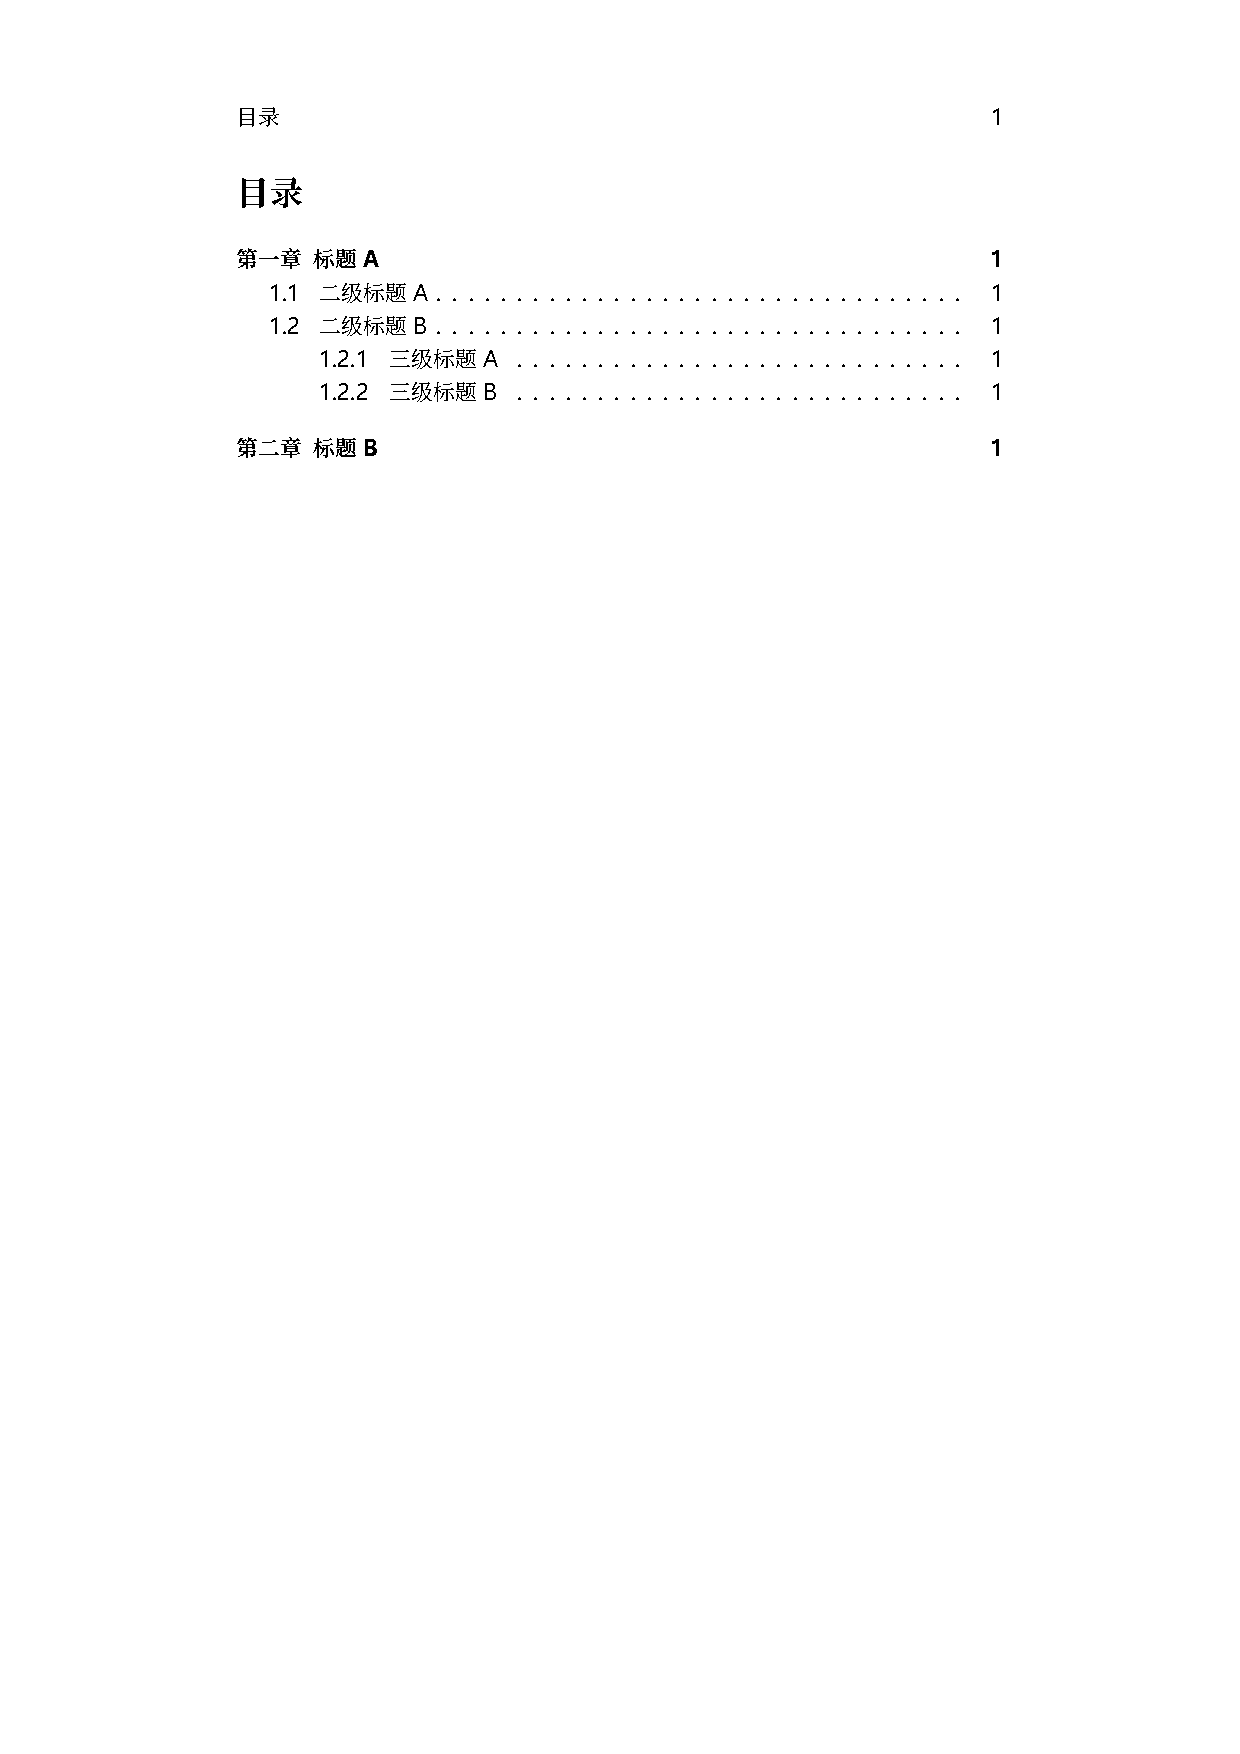
\includegraphics[page=1,clip,trim =0 {0.7\paperheight} 0 {0.1\paperheight},width=0.8\textwidth]{fig/section-tmp.pdf}
    %        \caption{Title}
    %        \label{fig:somthing}
        \end{figure}
    \end{texsepcode}
    \LaTeX{}需要编译两次\footnote{实际上所有的具有引用性质的内容都需要编译两次才可以正常的显示出来,另外有一些需要跨页的(如longtable),也需要多次的编译才可以正常的显示}才可以完整的将目录显示出来,因为\LaTeX{}必须通过第一遍编译获取所有目录的引用,才可以在下一次编译的时候添加新的目录。

    \subsection{定义目录深度}
    默认情况下目录只支持到\highunderline{subsubsection},如果需要增加目录深度,需要在序言位置就要使用以下的代码:
    
    \begin{texsepcode}
        \begin{texcodenoshad}
            \setcounter{tocdepth}{4}%设置目录级数
            \setcounter{secnumdepth}{4}%设置在几级目录前标记序号
        \end{texcodenoshad}
        \tcblower
        \begin{figure}[H]
            \centering
            \includegraphics[page=1,clip,trim =0 {0.7\paperheight} 0 {0.1\paperheight},width=0.8\textwidth]{\figpath{section-depth.pdf}}
        \end{figure}        
    \end{texsepcode}

    两行代码中的数字和\Ref{subsec:标题介绍}中备注的数字相同。

    数字的设置不必相同,互相并不矛盾,根据需要更改即可,其中\highunderline[hlyellow]{tocdepth}表明目录支持到几级深度,\highunderline[hlyellow]{secnumdepth}表明标题序号标记到几级深度。另外第一遍编译的时候可能会看到目录中增加了目录级数但是章节号并没有被添加,这是正常现象,完全更新会延迟到下一次编译。

    \subsection{添加标题引用}\label{sub:ref-in-title}
    使用\highunderline{hyperref}宏包后,生成的目录会自动添加到具体章节的链接和书签(如果没有该宏包则目录没有链接)。但是如果在文章内引用某章节,仍然需要为章节添加引用\footnote{该方法不局限于为章节添加引用,参考\Ref{sub:标签}}。

    为章节添加引用的方法是使用\highunderline{\textbackslash{}label{唯一标记}},该方法适用于任何你想引用某个位置的说明的地方,以本小节,其代码如下:
    \begin{texcode}
        \subsection{添加标题引用}\label{sub:ref-in-title}
    \end{texcode}

    在使用时,则需要使用\highunderline{\textbackslash{}ref}命令,如:
    \begin{texshow}
        在\ref{sub:ref-in-title}一节提到了如何对标题添加引用。
    \end{texshow}

    有时,不仅需要看到引用的序号,还想要知道相应的标题的名字。要完成这个需求,需要使用\highunderline{nameref}包:
    \begin{texshow}
        % \usepackage{nameref}
        如何对标题添加引用可以查看\ref{sub:ref-in-title}:\nameref{sub:ref-in-title}
    \end{texshow}

    如果嫌同时使用两个引用命令来完成上面的操作有些麻烦,可以通过重新定义一条引用命令\footnote{如何定义一条命令参考\Ref{sec:comm-envi}}的方法来合并引用(本手册即使用这种方法):
    \begin{texcode}
        \newcommand{\Ref}[1]{\ref{#1}:\nameref{#1}}
    \end{texcode}

    \begin{texshow}
        如何对标题添加引用可以查看\Ref{sub:ref-in-title}
    \end{texshow}
    
    
    \subsection{重新定义标题序号格式}
    有的时候会遇到需要自己定制标题序号的需求,对于中文环境和英文环境,相应的定制方式略有不同:

    \subsubsection{英文环境}
    英文环境,暂略(可以使用\highunderline{titlesec}系列宏包)
    % \todo{定义标题序号格式}
    \subsubsection{中文环境}
    中文环境要更改序号需要使用\highunderline{ctex}提供的命令,如下:
    \begin{texcode}
        \ctexset{
        section = {
            number = 第\chinese{section}章,
            format = \zihao{3}\bfseries,
        },
        subsection = {
            number = \arabic{section}.\arabic{subsection},
            format = \Large\bfseries
        },
        subsubsection = {
            number = \arabic{section}.\arabic{subsection}.\arabic{subsubsection},
            format = \Large\bfseries,
        },
    }
    \end{texcode}
    使用方法如上所示(这也是本手册使用的参数),每个级别的标题都可以分别自定义,其中\highunderline{number}表示序号的格式,相关的知识可以查看\Ref{subsub:number}的描述。\highunderline{format}表示每个标题的格式,相当于对每个标题添加什么样的命令。

    \subsection[更改目录标题]{更改目录中的标题文字}
    有的时候,因为标题过长,会导致目录不好看,这个时候,可以通过给标题添加参数的方式,定义显示在目录中的标题的内容。
    \begin{texcode}
        \section[短标题(显示在目录中的标题)]{长标题(显示在章节中的标题)}
        % 其他标题类方法同理
    \end{texcode}

    可以通过查看本节在目录和章节中的标题来认识其效果,其对应的代码为:
    \begin{texcode}
        \subsection[更改目录标题]{更改目录中的标题文字}
    \end{texcode}

    \subsection{取消标题序号}
    有的时候需要不显示标题的序号,只需要在命令后加$*$号即可。
    \begin{texcode}
        \section*{No Title Section}
    \end{texcode}

    但这时标题也不会出现的目录中,如果需要标题仍然在目录中出现需要在此处添加额外的声明,如下:
    \begin{texcode}
        \section*{No Title Section}\addcontentsline{toc}{section}{Title of the section} 
        %三个参数分别表示添加的位置是\highunderline{正文目录(toc)},级别是\highunderline{section},目录中显示的文字是\highunderline{Title of the section}
    \end{texcode}
    其中,\highunderline{\textbackslash{}addcontentsline}命令还可以用于添加其他类型的目录,如表格(第一个参数为\highunderline{lot}),图片(\highunderline{lof})等,但并不是很常用。

    \subsubsection*{取消标题序号的演示}\addcontentsline{toc}{subsubsection}{取消标题序号的演示} 
    使用代码如下,注意添加后会在目录中失去页码的引用:
    \begin{texcode}
        
        \subsubsection*{取消标题序号的演示}
        \addcontentsline{toc}{subsubsection}{取消标题序号的演示} 
    \end{texcode} % 标题和目录
    \section{文字样式}\label{sec:文字样式}
    \subsection{一般效果}
    \subsubsection{正常输入}
    在中文环境里,中文默认字体为宋体。
    \begin{texshow}
        普通文字\\
        normal text
    \end{texshow}
    \subsubsection{斜体}
    
    在中文环境里,中文默认的斜体效果是\textit{楷体}而不是倾斜。
    \begin{texshow}
        \textit{斜体文字}\\
        \textit{Italian text}
    \end{texshow}

    斜体实际上有两种,一种是italic,一种是slanted,其中italic指“倾斜的字体”,而slanted则是指“字体的倾斜”,有细微的差别:
    \begin{texshow}
        \textit{斜体文字}\textit{Italian text}\\
        \textsl{倾斜文字}\textsl{slanted text}
    \end{texshow}

    \subsubsection{加粗}
    在中文环境里,中文默认的加粗效果是\textbf{黑体}而不是宋体加粗。
    \begin{texshow}
        \textbf{加粗文字}\\
        \textbf{normal text}
    \end{texshow}
    \subsubsection{添加线}

    \LaTeX{}提供默认的下划线\highunderline{\textbackslash{}underline}但是有很多的缺点因此不推荐使用,推荐使用\highunderline{ulem}宏包中的命令,该宏包还提供了许多其他的修饰操作,列举如下:
    \begin{texshow}
        % \usepackage{ulem}
        \uline{下划线}\\
        \uuline{双下划线}\\
        \uwave{波浪线}\\
        \sout{中间删除线}\\
        \xout{斜删除线}\\
        \dashuline{虚线}\\
        \dotuline{加点}
    \end{texshow}

    \subsection{字号}
    一般可以使用以下几种字号大小
    \begin{texbreakshow}
    \tiny{tiny-极小}\\
    \scriptsize{scriptsize-代码大小}\\
    \footnotesize{footnotesize-脚注大小}\\
    \small{small-小}\\
    \normalsize{normalsize-正常}\\ %默认字号
    \large{large-大}\\
    \Large{Large-很大}\\
    \LARGE{LARGE-极大}\\
    \huge{huge-巨大}\\
    \Huge{Huge-很巨大}
    \end{texbreakshow}

    在\href{http://mirrors.ibiblio.org/CTAN/language/chinese/ctex/ctex.pdf}{CTex手册}里包含了这些字号对应的磅数以及中文环境中重新设置这些大小的命令。

    \subsection{字体}
    \LaTeX{}中,中文和英文环境各自的字体需要分别调整。首先介绍一下基本的字体分类:
    \subsubsection{基本字体类型}

    \paragraph{serif}
    即\textbf{衬线字体},指的是具有末端加粗、扩张或尖细末端,或以实际的衬线结尾的一类字体。

    serif 总是在文字末端做文章,这样做的目的是增强可读性,也就是说在字号比较小的时候,serif 一族的字体仍然是比较好辨认的。

    在\LaTeX{}中,衬线字体以罗马字族(Roman)的形式存在的。
    \paragraph{sans-serif}
    即\textbf{无衬线字体}。sans是法语前缀,意为“无”,在表意明确的情况下,可以称为sans。

    sans字体比较圆滑,线条粗线均匀,适合做艺术字、标题等,与“衬线字体”相比,如果字号比较小,看起来就会有些吃力。

    在\LaTeX{}中,无衬线字体以无衬线字族的形式存在。
%  BoldFont = SimHei , ItalicFont = KaiTi_GB2312
    \paragraph{monospace}
    即\textbf{等宽字体},有的字体不同的标点、英文字母、汉字宽度是不一样的,在显示代码的时候就需要使用这种字体,对齐后会很舒服。

    
    \subsubsection{字族}
    一个字族是指一组专门设计的、一起协调使用的字体。一般有正文,粗体,斜体,斜粗体四种组成,有时根据具体需要没有斜粗体也可以,有时还会出现超过四种字形的字族。

    \LaTeX{}默认有三种字族,分别叫做\highunderline{mainfont},表示一般的罗马字族,\highunderline{sansfont},表示无衬线字族,\highunderline{monofont},表示等宽字族。

    \subsubsection{字体设置}
    使用XeLaTeX编译可以使用电脑中的系统字体,而不只是使用\LaTeX{}的内置字体,所以这是目前使用XeLaTeX编译的一大原因。

    如果不添加\highunderline{cte}宏包,那么一般使用\highunderline{fontspec}宏包来完成字体(主要是英文字体)的设置;如果使用了\highunderline{ctex}宏包,那么中英文字体均可以使用ctex宏包提供的命令来设置,这里仅介绍使用ctex宏包的设置方法。按照本文的方法,基本能够满足日常使用,如果需要更高度的定制化,可以查看\highunderline{xecjk}、\highunderline{footspec}、\highunderline{cjk}宏包,ctex宏包的实现继承了这些宏包,因此在其文档中没有仔细解释如何使用这些命令。

    ctex宏包使用\highunderline{setxxxfont}设置英文字体族字体\footnote{这也是\highunderline{fontspec}宏包使用的方法},使用\highunderline{setCJKxxxfont}设置中文字体,中英文各有四种,分别是main(正文默认),sans(无衬线),mono(等宽),math(数学环境)
    以设置罗马字族的英文字体为例:
    \begin{texcode}
        \setmainfont[UprightFont=xxx,
             BoldFont=xxx,
             ItalicFont=xxx,
             BoldItalicFont=xxx,
             SmallCapsFont=xxx,
             SlantedFont=xxx}
            ]{Latin Modern Roman}
    \end{texcode}

    在大括号内设置整个字族的字体,但是有时候一个字体可能会缺少一些字形,如缺少斜体等,这个时候可以设置可选参数中的七个字形。

    下面介绍字体参数应该如何填入。
    \subsubsection{找到字体}
    如果使用XeLaTeX编译,那么就可以使用系统字体\footnote{其使用\highunderline{fontconfig}库查找和调用字体},否则只能使用在Tex安装目录下安装的字体。

    在命令行输入以下命令,可以在当前目录得到一个文本文件\footnote{由于汉字编码原因,Windows下总需要把字体列表输出的文件中防止乱码。},里面显示了所有可用的字体文件。
    \begin{languagebox}[bash]
        fc-list > fontlist.txt
    \end{languagebox}

    该命令也可以加上各种选项来进行筛选,如只需要列出所有中文字体\footnote{关键是其中的语言选项zh。日文使用ja,韩文使用ko,英文使用en},使用命令:
    \begin{languagebox}[bash]
        fc-list -f "%{family}\n" :lang=zh > zhfont.txt 
    \end{languagebox}

    一般,会得到如下的文字
    \begin{verbatim}
        C:/Windows/fonts/msyh.ttc: Microsoft YaHei,微软雅黑:
            style=Regular,Normal,obyčejné...
    \end{verbatim}

    或者这样的文字
    \begin{verbatim}
        FZYaoTi,方正姚体
        FandolSong
        SimHei,黑体
        Microsoft YaHei,微软雅黑
        STFangsong,华文仿宋
    \end{verbatim}
    可以直接使用字族名,或者文件名来设置字体,如:
    \begin{texcode}
        \setmainfont{Microsoft YaHei}
        \setmainfont[
            ItalicFont=STFangsong,
        ]{msyh.ttc}
    \end{texcode}

    
    \subsubsection{局部调整字体}
    其中,mainFont影响的是\highunderline{\textbackslash{}rmfamily}和\highunderline{\textbackslash{}textrm}命令的效果。\marginnote{xxfamily影响的是作用域内的,textxx影响的是命令内的参数}

    

    sansFont影响的是\highunderline{\textbackslash{}sffamily}和\highunderline{\textbackslash{}textsf}命令的效果。

    monoFont影响的是\highunderline{\textbackslash{}ttfamily}和\highunderline{\textbackslash{}texttt}命令的效果。
    \begin{texshow}
        \sffamily san文本开始的地方\\\texttt{mono文本}\textsf{sans文本}{\rmfamily roman文本}sans文本结束
    \end{texshow}

    \subsection{调整位置}
    如果需要将文字上下偏移,可以使用\highunderline{\textbackslash{}raisebox}
    \begin{texshow}
        正常文本 \raisebox{1cm}{提升文本} \raisebox{-1cm}{下降文本}正常文本
    \end{texshow}

    如果需要增加文字之间的间隙,可以使用\highunderline{\textbackslash{}hspace}
    \begin{texshow}
        正常文本\hspace{1em}正常文本\\
    \end{texshow}
    如果要填满空隙,可以使用\highunderline{\textbackslash{}hfill}:
    \begin{texshow}
        A \hfill A \hfill A \hfill A \\
        A \hspace{\stretch{2}} A \hfill A \hfill A \\
        A \hfill A \hfill A\hspace{0.5cm} A \hfill A \hfill A \hspace{0.5cm} A 
    \end{texshow}
    注意第三个示例,每个\highunderline{\textbackslash{}hfill}占用的宽度在计算后都是一样的,但是会减去其他的固定长度的宽度。

    另外,在数学公式中,需要使用其他的命令来帮助缩进(以下这些命令在普通环境也可以使用
    \begin{texshow}
        $a\qquad{}b$\\ % 两个quad空格,两个字符 "M" 的的宽度
        $a\quad{}b$\\ % quad空格,一个字符 "M" 的的宽度
        $a\ b$\\ % 大空格 1/3字符 "M" 的宽度
        $a\;b$\\ % 中等空格	2/7字符 "M" 的宽度
        $a\,b$\\ % 小空格 1/6字符 "M" 的宽度
        $ab$\\ % 没有空格
        $a\!b$ % 缩进1/6字符 "M" 的宽度
    \end{texshow}

    \subsection{上下标}
    在数学环境中,使用上下标可以通过简单的\highunderline{\_{}},\highunderline{\^{}}来实现,如下:
    \begin{texshow}
        $A^e_l,a_3,b^5$
        $A^{ext}_{ext}$ % 多个字母需要放在上下标中需要用花括号括起来
    \end{texshow}

    在普通环境中,不能直接使用数学环境中的方法,需要引入\highunderline{fixltx2e}包来实现文本环境中的上下标
    \begin{texshow}
        % \usepackage{fixltx2e}
        普通文本\textsubscript{下标文本}\textsuperscript{上标文本}
    \end{texshow}


    \subsection{特殊字符}
    \LaTeX 里存在一些特殊字符,如果需要在普通环境里使用,需要声明,具体的字符内容如下:
    \begin{center}
        \setlength\tablewidth{\dimexpr (\textwidth -20\tabcolsep)}
        \begin{table}[H]
            \begin{tabular}{|p{0.06\tablewidth}<{\centering}|p{0.06\tablewidth}<{\centering}|p{0.06\tablewidth}<{\centering}|p{0.06\tablewidth}<{\centering}|p{0.06\tablewidth}<{\centering}|p{0.06\tablewidth}<{\centering}|p{0.08\tablewidth}<{\centering}|p{0.08\tablewidth}<{\centering}|p{0.06\tablewidth}<{\centering}|p{0.41\tablewidth}<{\centering}|}
                \hline
                字符&\#&\%&\%&\{&\}&\~{}&\_{}&\&&\textbackslash\\
                \hline
                命令&\verb|\#|&\verb|\%|&\verb|\%|&\verb|\{|&\verb|\}|&\verb|\~{}|&\verb|\_{}|&\verb|\&|&\verb|\textbackslash{}|\\
                \hline
            \end{tabular}
        \end{table}
    \end{center}
    
    在数学环境中,直接使用小括号()和中括号[],可能会不太美观,可以使用\highunderline{\textbackslash{}left}和\highunderline{\textbackslash{}right}来使其具备自动调整大小的能力:
    \begin{texshow}
        $\left( foo \right)$
        $\left[ foo \right]$
        $\left( foo \right.$ %left 和 right命令必须成对出现,如果需要一边某有括号,可以将括号变成点来去掉相应位置的括号。
        $\left. foo \right]$ %left 和 right命令必须成对出现,如果需要一边某有括号,可以将括号变成点来去掉相应位置的括号。
    \end{texshow}
    另外注意:大括号不可以使用这两个命令,否则会编译报错。

    对于单双引号,正确用法是使用键盘左上角的反引号来表示左引号,靠紧L键的引号表示右引号,其中键入一个表示单引号,连续两个表示双引号(在中文环境中这种差异并不明显,主要是在英文环境中会存在问题):
    \begin{texshow}
        正确的`单引号'与``双引号''\\
        '英文中的单引号'\\
        "英文中的双引号"\\
        ‘中文中的单引号’\\
        “中文中的双引号”
    \end{texshow}

    % 参考自:https://blog.csdn.net/simple_the_best/article/details/52742303

    \subsection{标注拼音}
    可以使用\highunderline{xpinyin}宏包实现,具体方法略。

    \subsection{文字阴影}
    可以使用shadowtext宏包实现,具体方法略。
    
    \subsection{文字高亮}
    文字高亮推荐使用\highunderline{tcolorbox}实现,可定制性强。(包括带颜色的下划线,圆角高亮等,都可以使用该宏包来实现)。

\section{段落样式}\label{sec:段落样式}
    \subsection{段落间距}
    段落间距的相关设置,可以参考\Ref{sub:normal-page-dist}一节。

    \subsection{对齐}
    对齐分为左对齐、右对齐、居中、两端对齐和行尾的分散对齐

    \subsubsection{左对齐}
    \begin{texshow}
        \begin{flushleft}
            左对齐环境
        \end{flushleft}        
        \raggedright 左对齐声明
    \end{texshow}
    \subsubsection{右对齐}
    \begin{texshow}
        \begin{flushright}
            右对齐环境
        \end{flushright}        
        \raggedleft 右对齐声明
    \end{texshow}
    \subsubsection{居中}
    \begin{texshow}
        \begin{center}
            居中环境
        \end{center}        
        \centering 居中声明
    \end{texshow}
    这三种环境和相应的命令基本上能够在任意环境中嵌套并显示出相应的效果。

    % \linebreak 用于分散对齐
    \subsubsection{两端对齐}
    两端对齐需要使用\highunderline{ragged2e}宏包,并使用\highunderline{\textbackslash{}justifying}命令
    
        % 用于两端对齐的1文字用于a两端对齐b的文字用于两d端对齐的文字用e于两端对齐的文字用于两端对齐的文字用于两端对齐的文字用于u两端对t齐的文字用于两端对齐的文字f用于两端g对齐的文字用于两端对齐的文a字。
    
    % 对齐后的效果:
    % \begin{texshow}
        % \justifying{}用于两端对齐的1文字用于a两端对齐b的文字用于两d端对齐的文字用e于两端对齐的文字用于两端对齐的文字用于两端对齐的文字用于u两端对t齐的文字用于两端对齐的文字f用于两端g对齐的文字用于两端对齐的文a字。
    % \end{texshow}

    \subsubsection{分散对齐}
    分散对齐之前提到过,在换行的时候使用\highunderline{\textbackslash{}linebreak}即可:
    \begin{texshow}
        用于分散对齐的文字\linebreak
    \end{texshow}
    \subsection{环境的嵌套}

    一般情况位于\highunderline{document}环境中的文字均为普通文本,但是环境可以嵌套,被嵌套到特殊环境中的文字会从内到外依次根据所嵌套的环境产生相应的效果。如下图所示,使用了多个\highunderline{tcolorbox}互相嵌套后的效果:

    \begin{texshow}
        \begin{tcolorbox}[title=Outer box]
            \begin{tcolorbox}[title=Inner box]

                \begin{tcolorbox}[colframe=red,beforeafter skip=0pt]
                Deeply nested box using 60 percent of the available space.
                \end{tcolorbox}

                \begin{tcolorbox}[colframe=red,beforeafter skip=0pt]
                Deeply nested box using 40 percent of the available space.
                \end{tcolorbox}
            \end{tcolorbox}
        \end{tcolorbox}
    \end{texshow}

    \begin{quotation}
        该环境需要使用\highunderline{tcolorbox}包
    \end{quotation}


    \subsection{引文环境}
    引文环境为\highunderline{quotation},最多支持六级嵌套,效果如下:
    \begin{texshow}
        正常环境下的文字
        \begin{quotation}
            引文环境下的文字
            \begin{quotation}
                二级引文环境
            \end{quotation}
        \end{quotation}
        正常环境下的文字
    \end{texshow}
    \subsection{抄录环境}
    抄录环境为\highunderline{verbatim}会将所有的符号原封不动的继承下来:效果如下:

    \begin{texshow}
\begin{verbatim}
这是抄录环境!@#¥%……&*()(){}_+":>?
\end{verbatim}
    \end{texshow}

\subsection{普通边框}

如果要限制一行中文字的宽度,可以使用垂直盒子\highunderline{\textbackslash{}parbox}:
\begin{texshow}
    % \parbox[<position>]{<width>}{<text>},第一个参数一般省略,没有太多的使用场景。
    \parbox{5em}{示例文本示例文本示例文本示例文本示例文本示例文本示例文本示例文本示例文本}
\end{texshow}

对文字添加最普通的段落边框,使用内置的\highunderline{\textbackslash{}framebox}命令即可:

% \todo{看注释,盒子}
% https://zhuanlan.zhihu.com/p/24339981 

\begin{texshow}
    \framebox{示例文本示例文本示例文本示例文本示例文本示例文本示例文本示例文本示例文本示例文本示例文本示例文本示例文本示例文本示例文本示例文本示例文本示例文本示例文本示例文本示例文本示例文本示例文本示例文本示例文本示例文本示例文本示例文本示例文本示例文本}
\end{texshow}
遗憾的是直接使用framebox不能换行,如果要换行,可以再嵌套一层\highunderline{parbox}:
\begin{texshow}
    \framebox{
        \parbox{\textwidth-2\fboxsep-2\fboxrule}{示例文本示例文本示例文本示例文本示例文本示例文本示例文本示例文本示例文本示例文本示例文本示例文本示例文本示例文本示例文本示例文本示例文本示例文本示例文本示例文本示例文本示例文本示例文本示例文本示例文本示例文本示例文本示例文本示例文本示例文本}
    }
    \framebox{
        \parbox{\textwidth-4\fboxsep}{示例文本示例文本示例文本示例文本示例文本示例文本示例文本示例文本示例文本示例文本示例文本示例文本示例文本示例文本示例文本示例文本示例文本示例文本示例文本示例文本示例文本示例文本示例文本示例文本示例文本示例文本示例文本示例文本示例文本示例文本}
    }
\end{texshow}
\newpage

边框距离文字的间距用长度变量\highunderline{\textbackslash{}fboxsep}表示:
\begin{texshow}
    \setlength{\fboxsep}{0pt}
    \framebox{没有边框间隔}
\end{texshow}



\subsection{其他环境}
还有诗歌环境\highunderline{verse}等文档类自带的环境,使用方式大同小异。但实现各种段落样式的最佳实践是通过\highunderline{tcolorbox}来定义一个个盒子的样式。本书中所有的代码样例和边框等均依托于 tcolorbox 实现。 %普通文本
    \section{列表}\label{sec:列表}
    列表环境有三种,分别是\highunderline{itemize},\highunderline{enumerate},\highunderline{description}。
    \subsection{基本用法}
    生成没有序号的列表
    
    \begin{texshow}
        \begin{itemize}
            \item 第一个
            \item 第二个
            \item 第三个
            \begin{itemize}
                \item 第三个+1
                \item 第三个+2
            \end{itemize}
        \end{itemize}
    \end{texshow}
    
    生成有序号的列表
    \begin{texshow}
        \begin{enumerate}
            \item 第一个
            \item 第二个
            \item 第三个
            \begin{enumerate}
                \item 第三个+1
                \item 第三个+2
            \end{enumerate}
        \end{enumerate}
    \end{texshow}
    生成有标签描述的列表
    \begin{texshow}
        \begin{description}
            \item[itemize] 没有序号
            \item[enumerate] 有序号
            \begin{description}
                \item[罗马数字] 第一种
                \item[阿拉伯数字] ...
            \end{description}
            \item[description] 使用文字
        \end{description}
    \end{texshow}

    \subsection{自定义Bullet}
    "Bullet"是指各种List前的那个标记,中文译为"子弹",但觉得还是保留英文比较好一些。一般来说,默认的已经够用,但如果需要重新定义,\LaTeX{}同样支持高度可定制化的方式,另外,为了方便定制,可能需要使用\highunderline{enumitem}宏包\footnote{除了该宏包外,还有\highunderline{easylist},\highunderline{enumerate}等宏包可以完成,有需要可以自行了解}:
    \subsubsection{自定义标签}
    如果只是临时更改,那么只需要在\highunderline{\textbackslash{}item}后添加参数即可,如下:
    \begin{texshow}
        \begin{itemize}
            \item[--] 第一行
            \item[This] 第二行 %注意,虽然可以是文字,但缺少了description中的加粗,这是这两个环境的区别。
            \item 第三行 
        \end{itemize}
    \end{texshow}

    如果是统一更改一个itemize环境,那么可以在环境开始添加参数,如下:
    \begin{texshow}
        \begin{itemize}[label=--]
            \item 第一行
            \item 第二行
        \end{itemize}
    \end{texshow}

    如果是需要有一个经常使用的itemize环境,那么可以通过enumitem宏包直接定义一个,如定义一个\highunderline{todolist}(待完成列表):
    \begin{texshow}
        % \usepackage{enumitem}
        % \usepackage{amssymb} %\square 方法支持
        \newlist{todolist}{itemize}{2} % \newlist{<name>}{<type>}{<max-depth>}
        \setlist[todolist]{label=$\square$}
        
        \begin{todolist}
            \item 第一行
            \item 第二行
        \end{todolist}
    \end{texshow}

    上述的定义方法也可以合并为一个:
    \begin{texshow}
        \newlist{todolist2}{itemize}{2}
    \end{texshow}

    如果需要一个Bullet在多个环境里共用,那么可以新定义一个item,如下:
    \begin{texshow}
        \newcommand{\checkitem}{\item[$\square$]}%
        \begin{itemize}
            \item 第一行
            \checkitem 第二行
        \end{itemize}
    \end{texshow}

    我曾经因为需要定义了一个TOTOList,分享在这里:
    \begin{texshow}
        \begin{itemize}
            \item[$\square$]
            no checked
            \item[\rlap{\raisebox{0.3ex}{\hspace{0.4ex}\tiny \ding{52}}}$\square$]
            failed
            \item[\rlap{\raisebox{0.3ex}{\hspace{0.4ex}\scriptsize \ding{56}}}$\square$]
            checked
        \end{itemize}
    \end{texshow}
    \LaTeX{}中很难找到棱角分明的对号,只能用这种风格的折中一下。另外,关键在于Bullet如何用\LaTeX{}描述,如果需要很多使用,参考上面如何定义一个常用item。

    \subsubsection{自定义序号}
    序号的生成与\Ref{subsub:counter}和\Ref{subsub:number}有关,如果需要重新定义序号方式,方法与自定义标签类似,在单个item上重新定义需要借助计数器的名称,如:
    \begin{texshow}
        \begin{enumerate}
            \item 第一行 
            \stepcounter{enumi} % 如果指定了序号格式,需要使用之前手动对计数器加1
            \item[\alph{enumi}:] 第二行 
            \item 第三行 
            \begin{enumerate}
                \stepcounter{enumii}
                \item[\roman{enumii}] 二级+1
                \stepcounter{enumii}
                \item[\roman{enumii}] 二级+2 
            \end{enumerate}
        \end{enumerate}
    \end{texshow}

    在enumerate环境上的定义:
    \begin{texshow}
        \begin{enumerate}[label=\roman*)]
            \item 第一行
            \item 第二行
        \end{enumerate}
        \begin{enumerate}[label=\alph*--]
            \item 第一行
            \item 第二行
        \end{enumerate}
    \end{texshow}

    如果需要重新定义新的序号环境,方法同样与自定义标签类似:
    \begin{texshow}
        % \usepackage{enumitem}
        \newlist{romanlist}{enumerate}{2}
        \setlist[romanlist]{label=\roman*)}
        \begin{romanlist}
            \item 第一行
            \item 第二行
        \end{romanlist}
    \end{texshow}

    \subsection{版面与布局}
    \subsubsection{对齐与间隔}
    在使用\highunderline{enumitem}宏包后,就可以很方便的设置各种间距,有如下的几种:
    \begin{itemize}
        \item 垂直间距
        \begin{itemize}
            \item topsep
            \item partopsep
            \item parsep
            \item itemsep
        \end{itemize}
        \item 水平间距
        \begin{itemize}
            \item leftmargin
            \item rightmargin
            \item listparindent
            \item labelwidth
            \item labelsep
            \item itemindent
        \end{itemize}
    \end{itemize}
    
    可以通过附加参数的方式来设置,如:
    \begin{itemize}[itemsep=1ex, leftmargin=1cm]
        \item 示例文本示例文本示例文本示例文本示例文本示例文本
        \item 示例文本示例文本示例文本示例文本示例文本示例文本
    \end{itemize}
        
    如果要应用间隔设置到所有list,那么可以使用\highunderline{\textbackslash{}setlist}命令,如
    \begin{texshow}
        \newlist{romanlist}{enumerate}{2}
        \setlist[romanlist]{label=\roman*),leftmargin=1cm}
        \begin{romanlist}
            \item 第一行
            \item 第二行
        \end{romanlist}
    \end{texshow}
        
    \subsection{其他itemize布局}
    更多布局可以查看\href{https://en.wikibooks.org/wiki/LaTeX/List_Structures}{Wiki-List\_{}Structures} %列表
    \section{表格}\label{sec:table}
    \subsection{表格基础用法}
    
    单个的表格使用\highunderline{tabular}环境,一个最简单的表格如下所示:

    \begin{texshow}
        \begin{tabular}{cc} %% 有两个字母表示有两列,c 表示居中,还可以选择 l 或者 r
            A&B\\ % \\ 表示换行,&表示分割线
            C&D\\
        \end{tabular}
    \end{texshow}

    表格列数需要在参数中表明,行数不限制,使用\highunderline{ \textbackslash{}\textbackslash{} }换行即可。
    
    如果要添加边框(边框由分割线组成),对列添加分割线需要在参数中相应位置添加 "\textbar" ,对行分割线则使用 "\textbackslash{}hline" 或 "\textbackslash{}cline"
    \begin{texshow}
        \begin{tabular}{|cc||} % 因为右侧有两道线,所以相应位置显示两条分割线
            A&B\\\hline
            C&D\\\cline{0-1} %数字代表列数,从零开始,表示从 a-b 
            E&F\\\cline{0-0}
            G&H\\\cline{1-1} %边框可以任意重叠,但横向边框显示多条并不好控制,因此不推荐使用多条分割线完成特殊需求
            I&J\\\cline{0-0}\cline{1-1}
        \end{tabular}
    \end{texshow}
    
    \subsection{表格合并}

    有时后,会遇到合并表格的需求,合并表格需要使用\highunderline{multirow}这个库,并使用到\highunderline{\textbackslash{}multicolumn}和\highunderline{\textbackslash{}multirow}这两个方法,
    
    其中合并多列比较简单,在要合并的位置填入相应的命令,随后减少相应的分隔符即可
    \begin{texshow}
        \begin{tabular}{|c|c|c|c|c|}
            \hline
            1.0&2.0&3.0&4.0&5.0\\
            \hline
            6.0&\multicolumn{3}{c|}{合并三列}&7.0\\
            \hline
            8.0&9.0&10.0&11.0&12.0\\
            \hline
        \end{tabular}
    \end{texshow}

    合并多行同理,不过在相同列的位置需要空出来,并在设置分割线的时候将相应的列的位置空出来
    \begin{texshow}
        \begin{tabular}{|c|c|c|}
            \hline
            1.0&2.0&3.0\\
            \hline
            4.0&\multirow{3}{*}{合并三行}&5.0\\
            \cline{1-1}
            \cline{3-3}
            6.0&&7.0\\
            \cline{1-1}
            \cline{3-3}
            8.0&&9.0\\
            \hline
            10.0&11.0&12.0\\
            \hline
        \end{tabular}
    \end{texshow}

    如果要同时合并多行多列,则需要对两个命令嵌套使用:
    \begin{texshow}
        \begin{tabular}{|c|c|c|c|}
            \hline
            1.0&2.0&3.0&4.0\\
            \hline
            5.0&\multicolumn{2}{c|}{\multirow{3}{*}{合并三行两列}}&6.0\\
            \cline{1-1}
            \cline{4-4}
            7.0&\multicolumn{2}{c|}{}&8.0\\
            \cline{1-1}
            \cline{4-4}
            9.0&\multicolumn{2}{c|}{}&10.0\\
            \hline
            11.0&12.0&13.0&14.0\\
            \hline
        \end{tabular}
    \end{texshow}
    

    \subsection{表格列宽调整}
    表格如果不设置宽度,一列的字数如果太多,就有可能超出文档页面大小,变得很丑

    \begin{tabular}{|c|c|c|c|}
        \hline
        1.0&2.0&3.0&4.0\\
        \hline
        1.0&2.0&长文字示例长文字示例长文字示例长文字示例长文字示例长文字示例长文字示例长文字示例长文字示例长文字示例长文字示例长文字示例&4.0\\
        \hline
    \end{tabular}

    因此,需要固定表格大小,从而更好的控制表格,在综合了各个库的命令和用法后,认为使用\highunderline{tabular}环境中提供的参数p是最优的方式。
    
    \subsubsection{参数p}
    tabular的参数选项如下:
    \begin{texcode}
        \begin{tabular}[pos]{cols}
            ...
        \end{tabular}
    \end{texcode}
    其中[pos]大多数情况下可以忽略,而\{col\}的位置之前提到过可以填写clr表示居中、左对齐和右对齐。该位置还有一个可选参数为\highunderline{p\{wth\}},用于指明相应位置的列占据多大的列宽,如:

    \begin{texshow}
        \begin{tabular}{|c|c|p{3cm}|c|}
            \hline
            1.0&2.0&3.0&4.0\\
            \hline
            1.0&2.0&长文字示例长文字示例长文字示例长文字示例长文字示例长文字示例长文字示例长文字示例长文字示例长文字示例长文字示例长文字示例&4.0\\
            \hline
        \end{tabular}
    \end{texshow}
    被指明了列宽的列会自动换行,这种方式可以一般情况下的列宽过长的问题。但设置了这种方式后该列是默认左对齐的,如果要设置居中或者右对齐,需要利用该环境的附加命令。

    \subsubsection{tabular的附加命令}
    \highunderline{tabular}的参数中提供了以下附加命令,可以用于在相应列的每一个cell之前或者之后插入文字或命令,也即我们可以在文字前加入居中命令来实现当列的居中操作,如下:
    \begin{texshow}
        \begin{tabular}{|c|c|>{\centering}p{7cm}<{-insert}|c|}
            \hline
            1.0&2.0&3.0&4.0\\
            \hline
            1.0&2.0&长文字示例长文字示例长文字示例长文字示例长文字示例长文字示例长文字示例长文字示例长文字示例长文字示例长文字示例长文字示例&4.0\\
            \hline
        \end{tabular}
    \end{texshow}
    上面的示例为在第三列的每个元素前加入居中命令,并在之后插入字符串"-insert"

    \subsection{横置表格}
    % 横直表格使用\highunderline{rotating}环境中的\highunderline{sidewaystable}环境替代\highunderline{table}环境:
    横置表格可以使用\highunderline{adjustbox}宏包中的\highunderline{adjustbox}环境,指定旋转角度即可:
    \begin{texshow}
        % \usepackage{adjustbox}
        \begin{adjustbox}{angle=90}
            \begin{tabular}{|c|c|>{\centering}p{7cm}<{-insert}|c|}
                \hline
                1.0&2.0&3.0&4.0\\
                \hline
                1.0&2.0&长文字示例长文字示例长文字示例长文字示例长文字示例长文字示例长文字示例长文字示例长文字示例长文字示例长文字示例长文字示例&4.0\\
                \hline
            \end{tabular}
        \end{adjustbox}
    \end{texshow}


    \subsection{长表格}
    因为表格是一个盒子,因此无法分页,这样会导致长表格会挤在一页看不全,因此需要跨页表格的支持,搜索得到的方法有\highunderline{longtable}、\highunderline{supertabular}、\highunderline{xtab}等,在对比后,我认为使用\highunderline{longtable}相对来说更加方便,因此仅介绍使用\highunderline{longtable}\footnote{注意,longtable在使用中可能需要编译多次才能成型。}。

    \begin{texcode}
        \begin{center}
            % 注意,longtable中添加居中需要多使用一个\arraybackslash命令,否则会报错
            \begin{longtable}{|l|l|>{\centering\arraybackslash}p{0.4\columnwidth}|}%
                    \hline%
                    \multicolumn{3}{r}{Continued on Next Page}\\%
                    \hline%
                \endfoot% 此语句之前均为分页时的结尾行
                    \hline%
                    \multicolumn{3}{r}{Not Continued on Next Page}\\%
                    \hline%
                \endlastfoot% 此语句之前均为最后一页的结尾行
                \hline
                header 1&header 2&header 3\\%标题
                \hline
                Content1&9&Longer String\\%
                Content1&9&Longer String\\%
                Content1&9&Longer String\\%
                Content1&9&Longer String\\%
                ...
                Content1&9&Longer String\\%
            \end{longtable}%
        \end{center}
    \end{texcode}
    \begin{center}
        \begin{longtable}{|l|l|>{\centering\arraybackslash}p{0.4\textwidth}|}%
            % \endhead%
            \hline%
            \multicolumn{3}{r}{Containued on Next Page}\\%
            \hline%
            \endfoot%
            \hline%
            \multicolumn{3}{r}{Not Containued on Next Page}\\%
            \hline%
            \endlastfoot%
            \hline
            header 1&header 2&header 3\\%
            \hline
            Content1&9&Longer String\\%
            Content1&9&Longer String\\%
            Content1&9&Longer String\\%
            Content1&9&Longer String\\%
            Content1&9&Longer String\\%
            Content1&9&Longer String\\%
            Content1&9&Longer String\\%
            Content1&9&Longer String\\%
            Content1&9&Longer String\\%
            Content1&9&Longer String\\%
            Content1&9&Longer String\\%
            Content1&9&Longer String\\%
            Content1&9&Longer String\\%
            Content1&9&Longer String\\%
            Content1&9&Longer String\\%
            Content1&9&Longer String\\%
            Content1&9&Longer String\\%
            Content1&9&Longer String\\%
            Content1&9&Longer String\\%
            Content1&9&Longer String\\%
            Content1&9&Longer String\\%
            Content1&9&Longer String\\%
            Content1&9&Longer String\\%
            Content1&9&Longer String\\%
            Content1&9&Longer String\\%
            Content1&9&Longer String\\%
            Content1&9&Longer String\\%
            Content1&9&Longer String\\%
            Content1&9&Longer String\\%
            Content1&9&Longer String\\%
            Content1&9&Longer String\\%
            Content1&9&Longer String\\%
            Content1&9&Longer String\\%
            Content1&9&Longer String\\%
        \end{longtable}%
    \end{center}



    \subsection{表格美化}\label{table-beauty}
    对表格的美化,主要涉及列宽的调整和颜色的设置,列宽的调整先前的章节已经介绍,关于颜色的设置,参考\Ref{sssec:color-table}

    在表格下如果要设置边框和背景色,需要为xcolor添加table参数
    
    
    
    \begin{texcode}\usepackage[table]{xcolor}\end{texcode}
    \begin{texshow}
        \begin{tabular}{lllll}
            \toprule
            \emph{name} & \emph{foo} &&&  \\\midrule
            Models    & A  & B  & C  & D  \\
            \rowcolor{blue!50} Model $X$ & X1 & X2 & X3 & X4\\
            \rowcolor{green!50} Model $Y$ & Y1 & Y2 & Y3 & Y4\\\bottomrule
            \hline
        \end{tabular}
    \end{texshow}
    
    如果需要单独设置一列、边框、单个单元格的颜色,可以查阅\highunderline{colortbl}宏包。

    \subsection{添加表格说明}
    需要使用\highunderline{table}环境,并使用\highunderline{\textbackslash{}caption{}}命令,具体可以参考\Ref{subsub:float-caption}对\highunderline{float}环境的说明。

    \begin{texshow}
        \begin{center}
            \begin{table}[H]
                \begin{tabular}{|c|c|}
                    \hline
                    1.0&2.0\\
                    \hline
                \end{tabular}
                \caption{表格说明}
            \end{table}
        \end{center}
    \end{texshow}

    \subsection{自动生成表格工具}

    自动生成表格的工具网上有很多开源实现,推荐以下几种:
    \subsubsection{Tables Generator}
    网站链接:\href{http://www.tablesgenerator.com/latex_tables}{Tables Generator}

    该网站提供了一个通用的表格转换工具,在其提供的表格环境中填写好后,可以转换为多种格式下的表格代码,其中包括了\LaTeX{}。

    \begin{figure}[H]
       \centering
       \includegraphics[width=0.8\textwidth]{\figpath{table-generator.png}}
       \caption{Table-Generator网站截图}
       \label{fig:table-generator}
    \end{figure}



    \subsubsection{LatexTool}
    网站链接:\href{https://github.com/sailist/LatexTool}{LatexTool}
    
    是我写的一个Python工具,因为要考虑列宽,合并表格等,在网上找的众多工具并不能符合我的需求,于是用Python写了一个,目前基本能够实现我的需求,使用方法也比较简单。
    \begin{languagebox}[python]
        % 直接使用pip安装:pip install x2t
        % 可以直接使用控制台命令:x2t test.xlsx test.xls
        from LatexTool.ast import tabel

        if __name__ == '__main__':
            # tab = tabel.Tabel("../test.xlsx",center=False,fill=False)
            tab = tabel.Tabel("../test.xlsx")
            print(tab.to_tex())
    \end{languagebox}

    完美支持合并多行多列:
    \begin{texshow}
        \begin{tabular}{|c|c|c|c|}
            \hline
            \multicolumn{3}{|c|}{合并三列}&0.0\\
            \hline
            C&D&H&1.0\\
            \hline
            \multirow{2}{*}{合并两行}&F&\multicolumn{2}{c|}{\multirow{3}{*}{合并三行两列}}\\
            \cline{2-2}
            &K&\multicolumn{2}{c|}{}\\
            \cline{1-2}
            M&N&\multicolumn{2}{c|}{}\\
            \hline
        \end{tabular}
    \end{texshow}
    
    也可以将大小填充到整个页面,并设置居中:
    \begin{texshow}
        \begin{center}
            % \newlength\tablewidth % if haven't define the length 'tablewidth'
            \setlength\tablewidth{\dimexpr (\textwidth -8\tabcolsep)}
            \begin{table}[H]
                \begin{tabular}{|p{0.29\tablewidth}<{\centering}|
                    p{0.07\tablewidth}<{\centering}|
                    p{0.43\tablewidth}<{\centering}|
                    p{0.21\tablewidth}<{\centering}|}
                    \hline
                    \multicolumn{3}{|c|}{合并三列}&0.0\\
                    \hline
                    C&D&H&1.0\\
                    \hline
                    \multirow{2}{*}{合并两行}&F&\multicolumn{2}{c|}{\multirow{3}{*}{合并三行两列}}\\
                    \cline{2-2}
                    &K&\multicolumn{2}{c|}{}\\
                    \cline{1-2}
                    M&N&\multicolumn{2}{c|}{}\\
                    \hline
                \end{tabular}
            \end{table}
        \end{center}
    \end{texshow}

    % 参考文献:https://en.wikibooks.org/wiki/LaTeX/Tables


    
     %表格
    \section{图片}\label{sec:graphics}
    插入图片使用的命令是\highunderline{\textbackslash{}includegraphics[参数]\{图片路径\}},在添加包支持后,可以支持eps、png、jpg、pdf等多种格式,推荐使用png和eps两种格式的图片

    \begin{quotation}
        本手册用于说明的图片均来源于免费素材网站\href{https://pixabay.com/zh/}{pixabay},之后不再说明。        
    \end{quotation}
    \subsection{基本使用}
    \begin{texshow}
        \includegraphics{contents/fig/mosque.jpg}
    \end{texshow}
    
    如上图所示,有时会会遇到图片过大的情况,因此需要加入参数调整图片的大小,因为\highunderline{\textbackslash{}columnwidth}是去掉了各种页边距后并考虑了分栏时的当前页面宽度,因此一般以该宽度作为基准调整图片大小:
    \begin{texshow}
        \includegraphics[width=0.5\columnwidth]{contents/fig/mosque.jpg} % 具体大小根据图片宽高比调整小数即可
    \end{texshow}

    如果是长条形图片,则可以使用\highunderline{\textbackslash{}textheight}调整图片高度的形式来适应页面。
    \begin{texshow}
        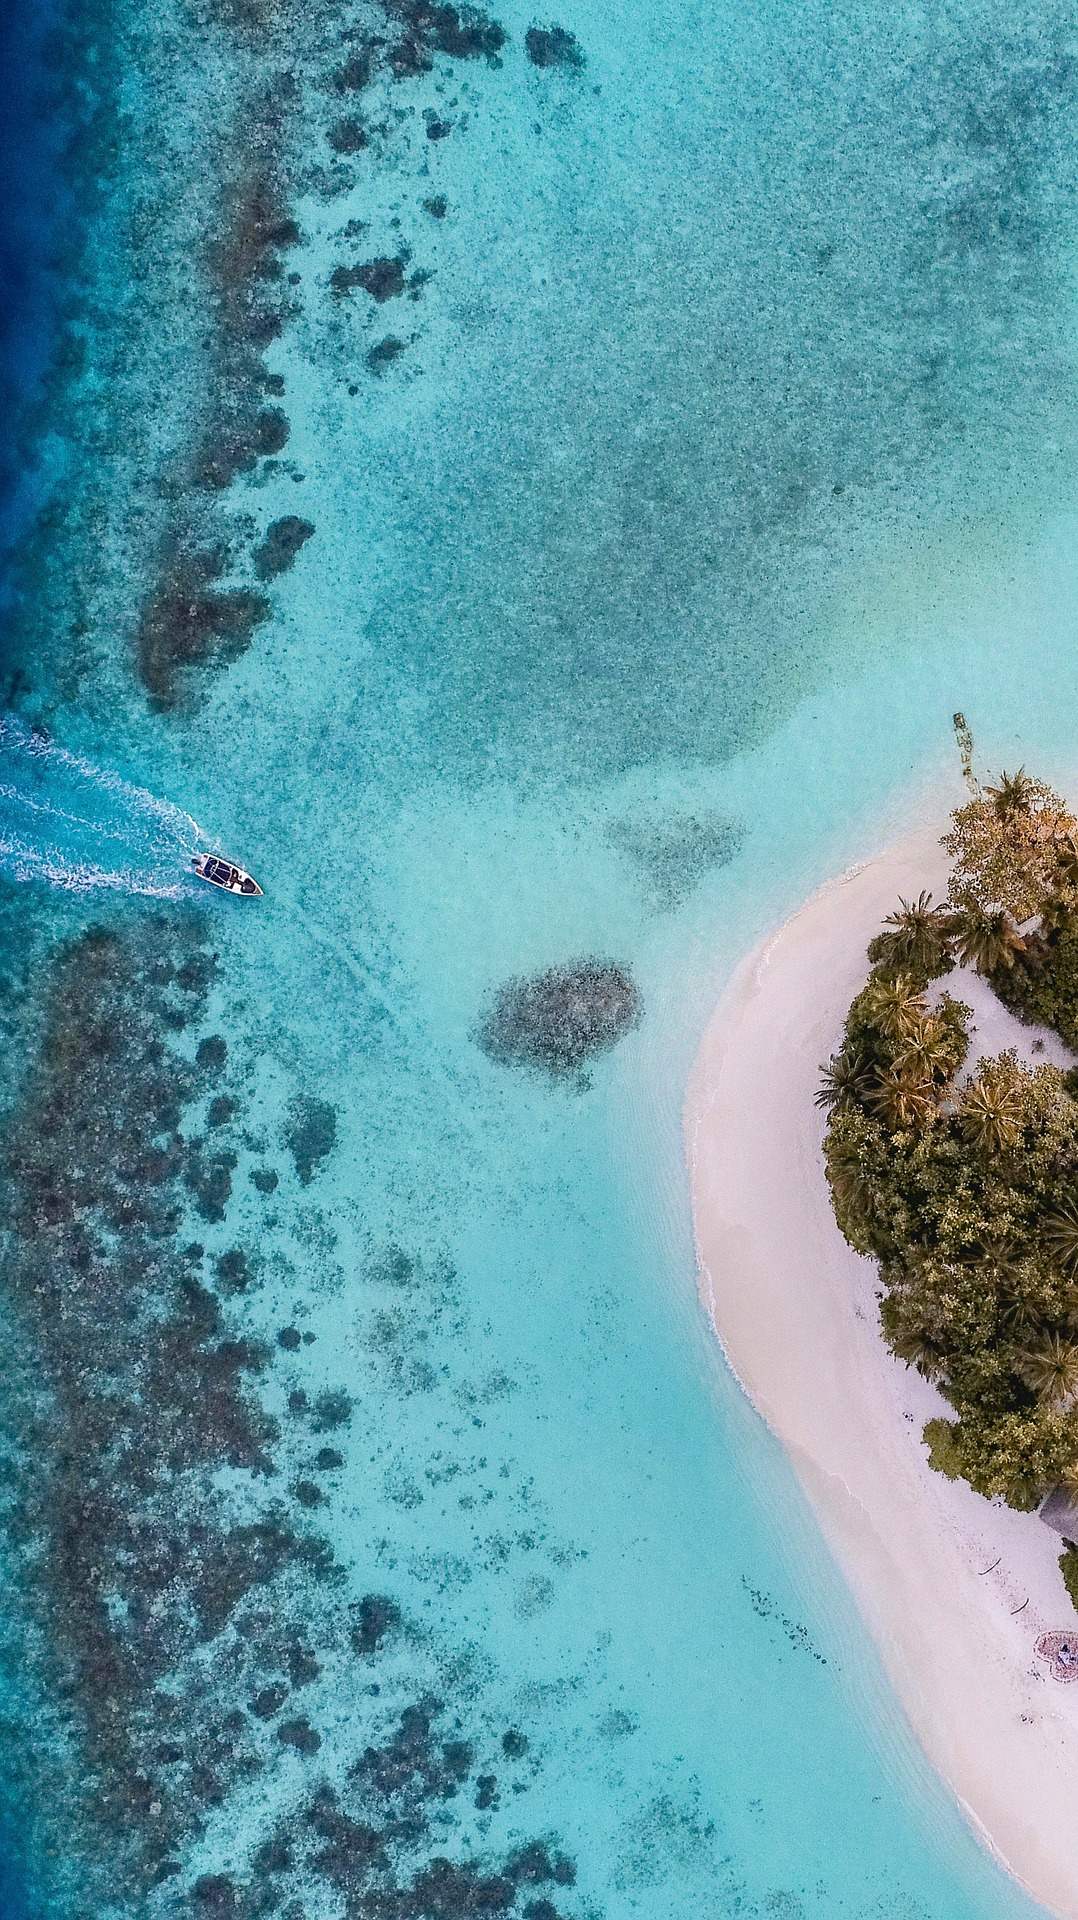
\includegraphics[height=0.4\textheight]{contents/fig/ocean.jpg}
    \end{texshow}

    注意,一般不同时调整图片长和宽,因为会导致图片失真。同时该命令还有\highunderline{scale}(缩放)参数(直接指定数字,不需要单位),但也一般不使用,因为在图片大小不统一的情况下,不便控制缩放比例。

    如果需要旋转图片,则使用\highunderline{angle}参数,直接指定数字表示度数
    \begin{texshow}
        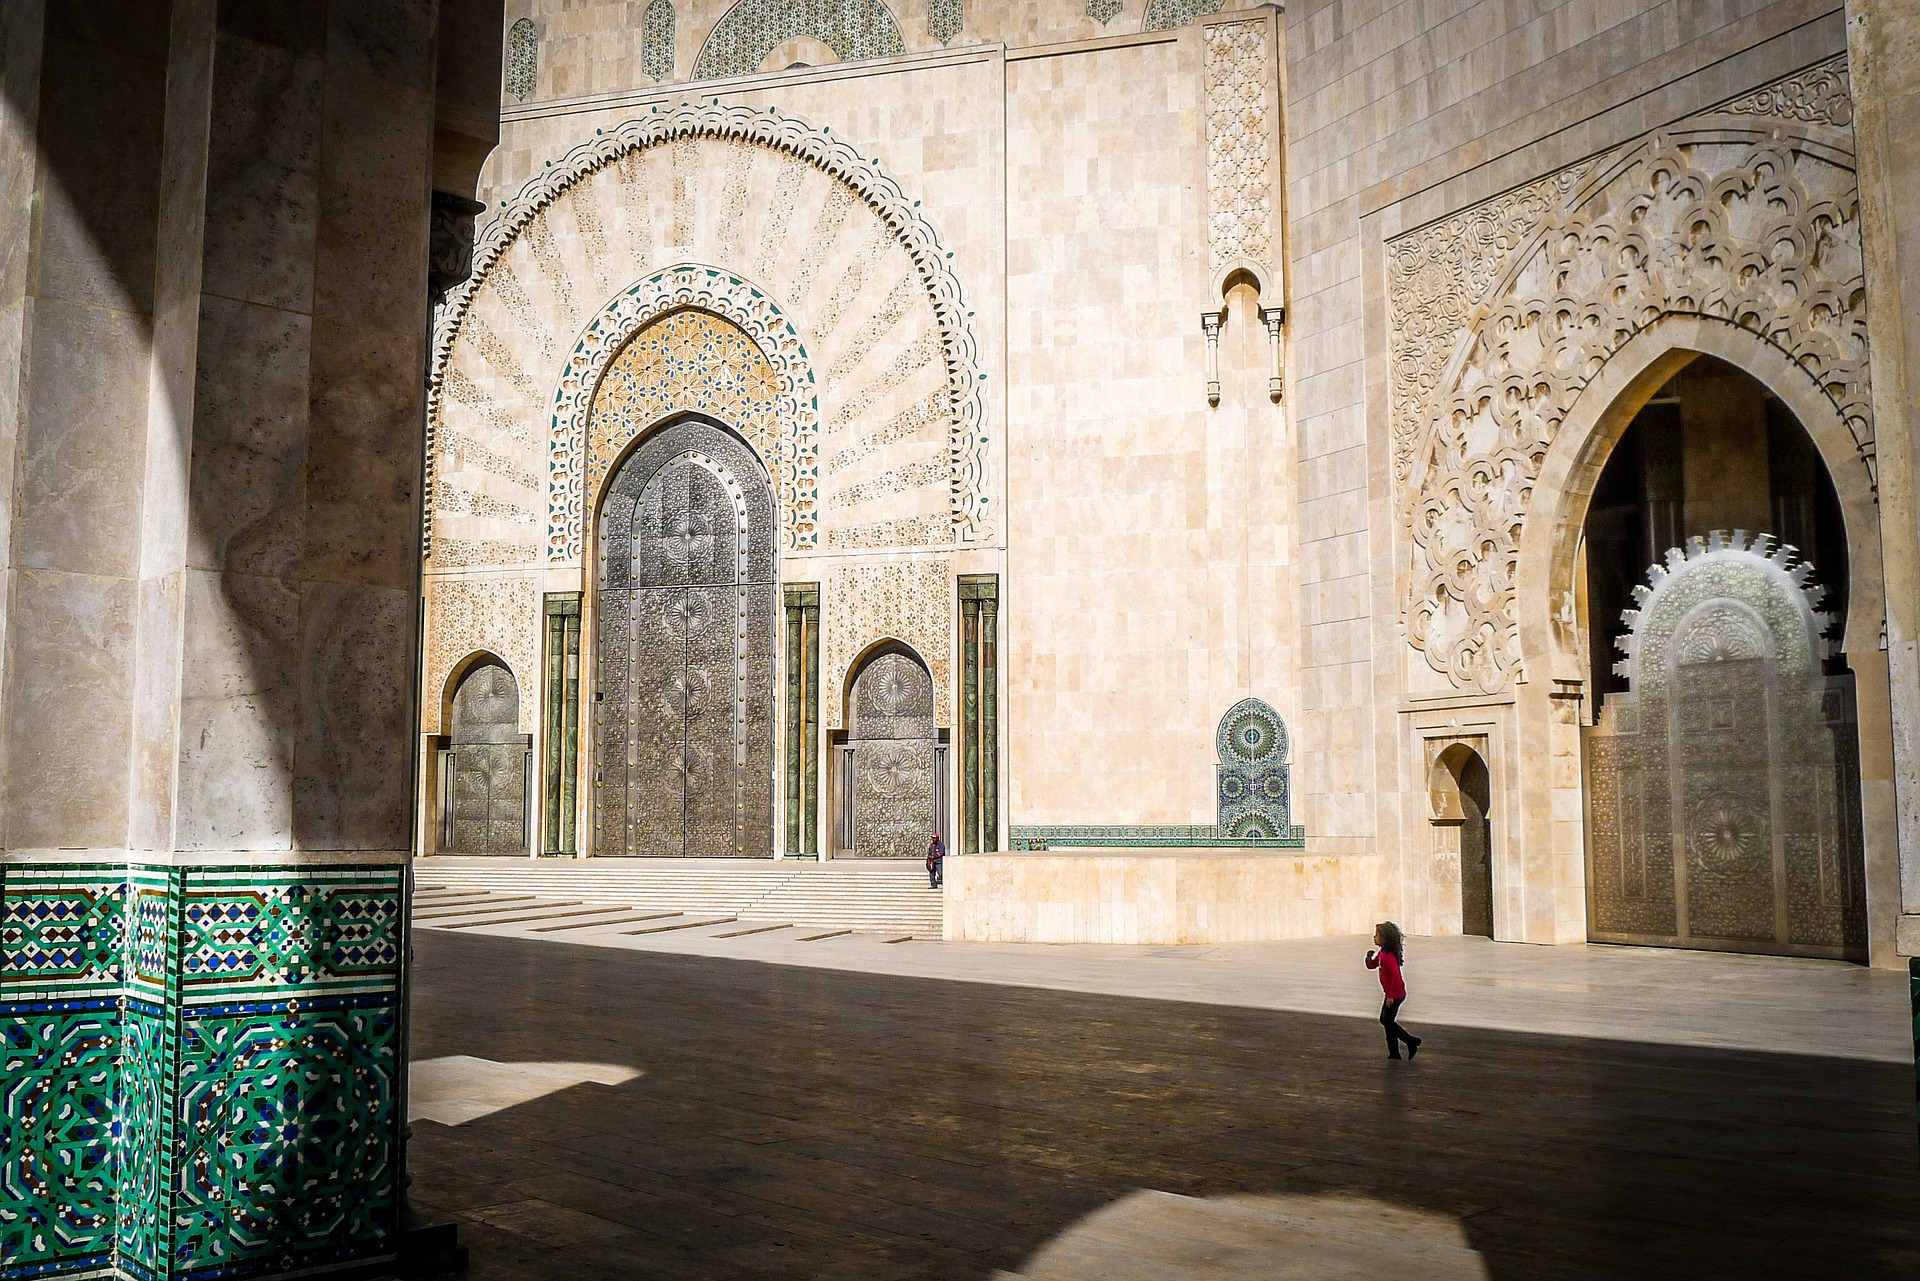
\includegraphics[width=0.3\columnwidth,angle=45]
                        {contents/fig/mosque.jpg}
        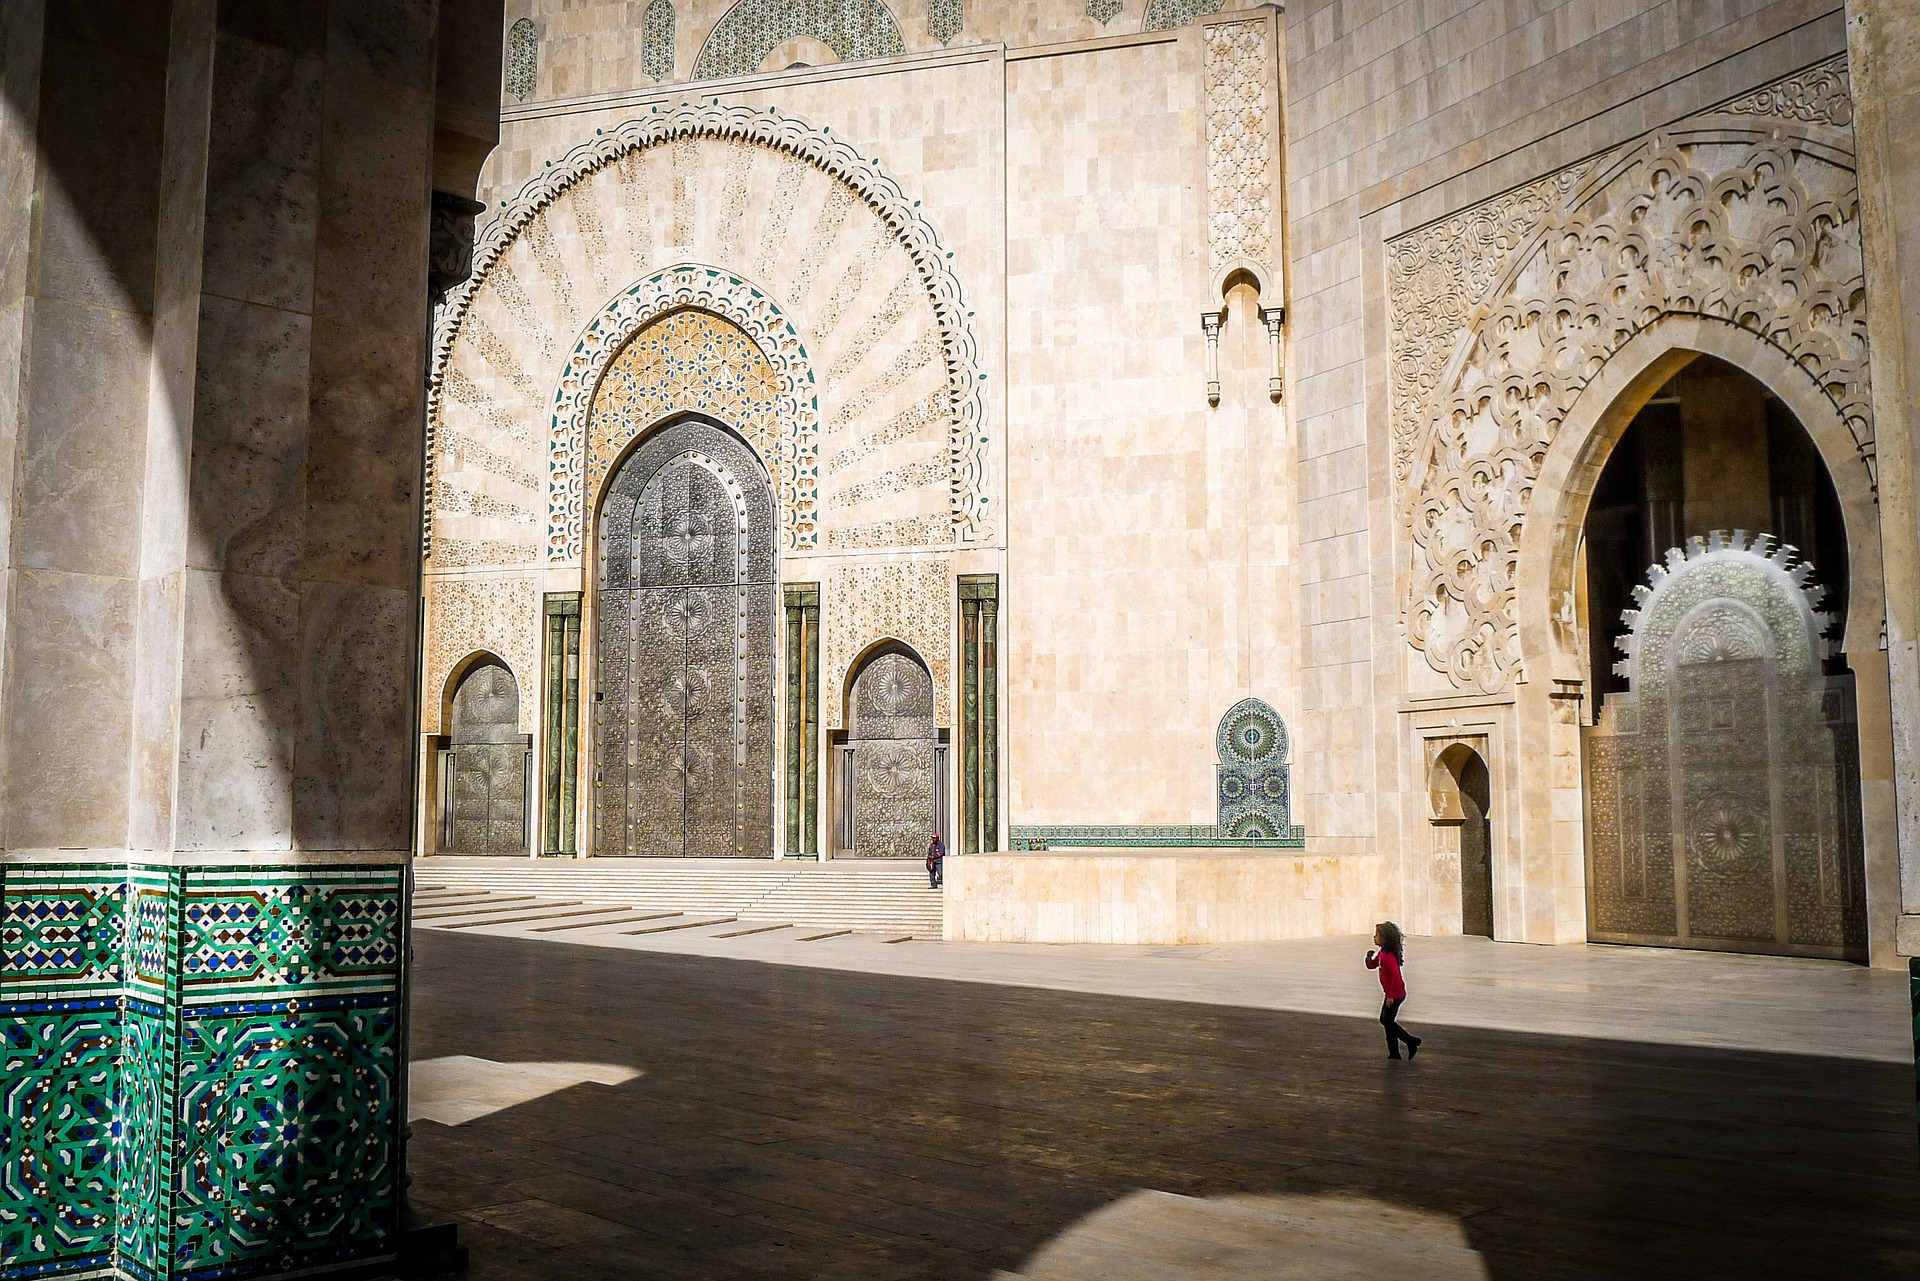
\includegraphics[width=0.3\columnwidth,angle=-45]
                        {contents/fig/mosque.jpg}
    \end{texshow}

    如果是添加PDF文档,可能会存在多页的问题,需要使用\highunderline{page}参数:

    \begin{texshow}
        \includegraphics[page=2,height=0.4\textheight]
                        {./contents/fig/section-depth.pdf}
    \end{texshow}

    如果要裁剪,则需要使用\highunderline{clip}和\highunderline{trim}参数,clip参数声明该图片需要裁剪(如果不声明则trim参数无效),trim则指明裁剪的边界:
    \begin{texshow}
        % 参数用法:trim = <left> <lower> <right> <upper>
        \includegraphics[clip,trim =2cm {0.4\paperheight} 2cm {0.4\paperheight},width=0.3\columnwidth]{contents/fig/mosque.jpg}\\
        \vspace{0.3\columnwidth}\\
        \includegraphics[width=0.3\columnwidth]{contents/fig/mosque.jpg}
    \end{texshow}
    \begin{quotation}
        注意,如果是直接指明长度,则不需要加\{...\}将长度包裹起来,如果是带有运算性质的长度,那么则需要用\{...\}将长度包裹起来,否则无法识别。
    \end{quotation}

    \subsection{指明图片路径}
    \highunderline{\textbackslash{}includegraphics}命令支持相对路径(\LaTeX{}编译时路径)和绝对路径两种路径,但即使是相对路径,有时也会因为更改而导致目录失效,因此可以以下命令指明图片目录,从而在插入图片时候只需要添加图片名字即可。

    \begin{texcode}
        \graphicspath{{./}{./contents/}{./contents/fig/}}%设置图片可能存在的路径
    \end{texcode}

    设置后\LaTeX{}编译时会自动寻找目录下的图片。

    \subsection{图片优先级读取}
    如果不加扩展名,编译时会依次寻找同名且为图片格式后缀的文件,在序言区声明以下内容可以更改其优先级。
    \begin{texcode}
        \DeclareGraphicsExtensions{.eps,.png,.jpg}%对于同名图片的优先顺序调用
    \end{texcode}

    \subsection{添加图片说明}
    参考\Ref{sub:figure}一节对\highunderline{Figure}环境的说明。

    \subsection{Tikz绘图}
    \LaTeX{}内内置了绘图方法,可以直接绘制出矢量图,\href{http://www.texample.net/tikz/examples/all/}{TikZ and PGF examples}网站上提供了大量精美(或复杂)的Tikz绘图示例:
    \begin{figure}[H]
       \centering
       \includegraphics[width=0.8\textwidth]{\figpath{tikzexample.png}}
       \caption{TikZ and PGF examples网站截图}
       \label{fig:tikzexample.png}
    \end{figure}
    使用Tikz的一个示例如下:
    \begin{texshow}
        \begin{tikzpicture} 
            \draw[step=1,color=gray!40] (-2,-2) grid (2,2); 
            \draw[->] (-3,0) -- (3,0);
            \draw[->] (0,-3) -- (0,3); 
            \draw (0,0) circle (1);  
        \end{tikzpicture}     
    \end{texshow}
    理论上Tikz可以绘制出你想要的任何图片,但是实际上由于该宏包过于复杂,除了技术狂魔外我不推荐直接使用内置的Tikz宏包来绘制矢量图...而是通过其他的手段(如Adobe Illustrator,Matplotlib)导出矢量图后以图片的形式添加,因此这里仅仅简单的介绍一下Tikz,具体的使用略。

 %图片
    \section{公式环境}\label{sec:公式}
    行内公式、行间公式、下标显示、label添加、公式编辑工具

    公式环境也叫做数学环境,是用来处理各种各样的数学符号的,并且支持多种展示属性,一般情况下,使用\highunderline{amsmath}包即可
    

    \subsection{行内公式}
    行内公式可以使用\highunderline{math}环境,\verb|\(..\)|或者\verb|$...$|三种方法:

    \begin{texshow}
        % \usepackage{amsmath}
        正常文本嵌套行内公式A:\begin{math}f_i(x)=a+b\end{math}。\\
        正常文本嵌套行内公式B:\(f^2(x)=a*b\)。\\
        正常文本嵌套行内公式C:$g(l;\theta)=a-b$。
    \end{texshow}

    \subsubsection{数学环境中的普通文本}
    如果要在公式内添加解释文本,英文可以直接支持,但是会转换成公式默认字体(itali斜体),并且不支持中文输入,因此如果要在公式环境内添加解释,需要使用\highunderline{amsmath}包中的\highunderline{\textbackslash{}text}命令:
    \begin{texshow}
        $g(l;\theta)=a-b,\text{正常文本 normal text},正常文本 normal text$
    \end{texshow}

    \subsection{行间公式}
    首先一定要注意,\textbf{行间公式不能有空行}!所以每一条公式必须紧靠着。如果要换行,需要使用\verb|\\|声明(仅在\textbf{多行公式}环境中有效)。
    
    \subsubsection{单行行间公式}
    单行行间公式不支持换行符(会忽略换行符)。

    如果不需要对行间公式进行编号,可以直接使用\verb|\[...\]|或\verb|$$...$$|
    \begin{texshow}
        公式前文本
        \[
            x = a+b;\\
            y = c+d;
        \]
        公式后文本
    \end{texshow}

    如果需要对一整个行间公式进行编号,可以使用\highunderline{equation}环境:
    \begin{texshow}
        \begin{equation}
            x = a+b;\\
            y = c+d;
        \end{equation}
    \end{texshow}

    \subsubsection{多行行间公式}
    如果要分段定义编号,可以使用\highunderline{eqnarray}环境,会对每一部分单独编号,如果不需要编号,在当前行添加\highunderline{\textbackslash{}nonumber}:
    \begin{texshow}
        \begin{eqnarray}
            x = a+b;\\
            y = c+d;\nonumber\\
            z = e+f;
        \end{eqnarray}
    \end{texshow}
    如果要对多个公式单独编号,但有对其中几个公式完成组编号,可以在公式中嵌套\highunderline{split}环境(注意在环境结束后添加换行符):
    \begin{texshow}
        \begin{eqnarray}
            \begin{split}
                a = 1;\\
                b = 2;\\
                c = 3;\\
            \end{split}\\
            x = a+b;\\
            y = c+d;\nonumber\\
            z = e+f;
        \end{eqnarray}
    \end{texshow}
    如果要重新开始编号或从指定数字开始编号,使用\highunderline{\textbackslash{}setcounter\{equation\}\{1\}}方法。

    \begin{texshow}
        \begin{eqnarray}
            \setcounter{equation}{2}
            \begin{split}
                a = 1;\\
                b = 2;\\
                c = 3;\\
            \end{split}\\
            \setcounter{equation}{7}
            x = a+b;\\
            y = c+d;\\
            z = e+f;
        \end{eqnarray}
    \end{texshow}

    如果需要对齐,则使用\highunderline{align}环境,并在要对齐的地方使用\&声明:
    \begin{texshow}
        \begin{align}
            &f(x) = a+b+c;\\
            g(x) = a;&
        \end{align}
    \end{texshow}
    同时,在\highunderline{eqnarray}环境中可以直接使用\highunderline{align}的方式进行对齐

    \subsection{公式编辑工具推荐}
    \subsubsection{Mathpix}
    网站链接:\href{https://mathpix.com/}{Mathpix}。

    如果有图片类型的公式,可以用该软件截图生成\LaTeX{}公式,多平台支持,且准确率很高,即使多行公式也能有很高的准确率,同时免费用户每天有50次截图的限额,非常划算。
    \begin{figure}[H]
       \centering
       \includegraphics[width=0.8\columnwidth]{\figpath{mathpix.png}}
       \caption{Mathpix官网示例}
       \label{fig:mathpix}
    \end{figure}


    \subsubsection{在线\LaTeX{}公式编辑器}
    网站链接:\href{https://www.codecogs.com/latex/eqneditor.php}{eqneditor}

    网站丑了点,但是能够对公式进行所见即所得的编辑,比较友好,目前暂时没有找到比它更好的替代方案,不过如果配置时使用的是Tex专门的IDE,其公式编辑应该也比较方便(不过可能不支持所见即所得) %公式环境
    \section{Float}\label{sec:Float}
    \subsection{Float基本介绍}    
    \highunderline{Float}是一类环境,指的是放置位置不固定的内容,如表格或图片,有时如果强行插入在当前段落,可能会造成空白,因此可以适当的在后续的几页中放置,但如果靠自己调整,一定是十分麻烦,因此便Float环境,它可以自动的寻找合适的位置插入。一般来说,Float环境支持五种参数,如下:
    \begin{center}
        % \newlength\tablewidth % if haven't define the length 'tablewidth'
        \setlength\tablewidth{\dimexpr (\textwidth -4\tabcolsep)}
        \begin{table}[H]
            \begin{tabular}{|p{0.09\tablewidth}<{\centering}|p{0.91\tablewidth}<{\centering}|}
                \hline
                h&将Float尽可能的放在当前位置(here),注意是尽可能,如果放不下,可能还是会放在别的位置\\
                \hline
                t&放在一页的顶部(Top)\\
                \hline
                b&放在一页的底部(Bottom)\\
                \hline
                p&放在一个特定的放Float的位置\\
                \hline
                !&重写\LaTeX{}内置的对于“好”的Float位置的偏好。\\
                \hline
                H&将Float环境准确的放到该位置,相当于只使用Float提供的其他特性,不使用Float的“浮动”特性,使用该参数需要使用\highunderline{float}包。\\
                \hline
            \end{tabular}
            \caption{Float的参数}
            \label{tab:float-param}
        \end{table}
    \end{center}

    \begin{quotation}
        在后续的使用中,为了方便演示,一律使用\highunderline{H}参数,其他参数的效果请读者自行试验。
    \end{quotation}

    \subsubsection{添加Float说明}\label{subsub:float-caption}
    通过在Float环境中使用\highunderline{\textbackslash{}caption\{描述\}}命令,可以为该Float添加描述,如图:

    \begin{texsepcode}
        \begin{texcodenoshad}
            \begin{figure}[H]
                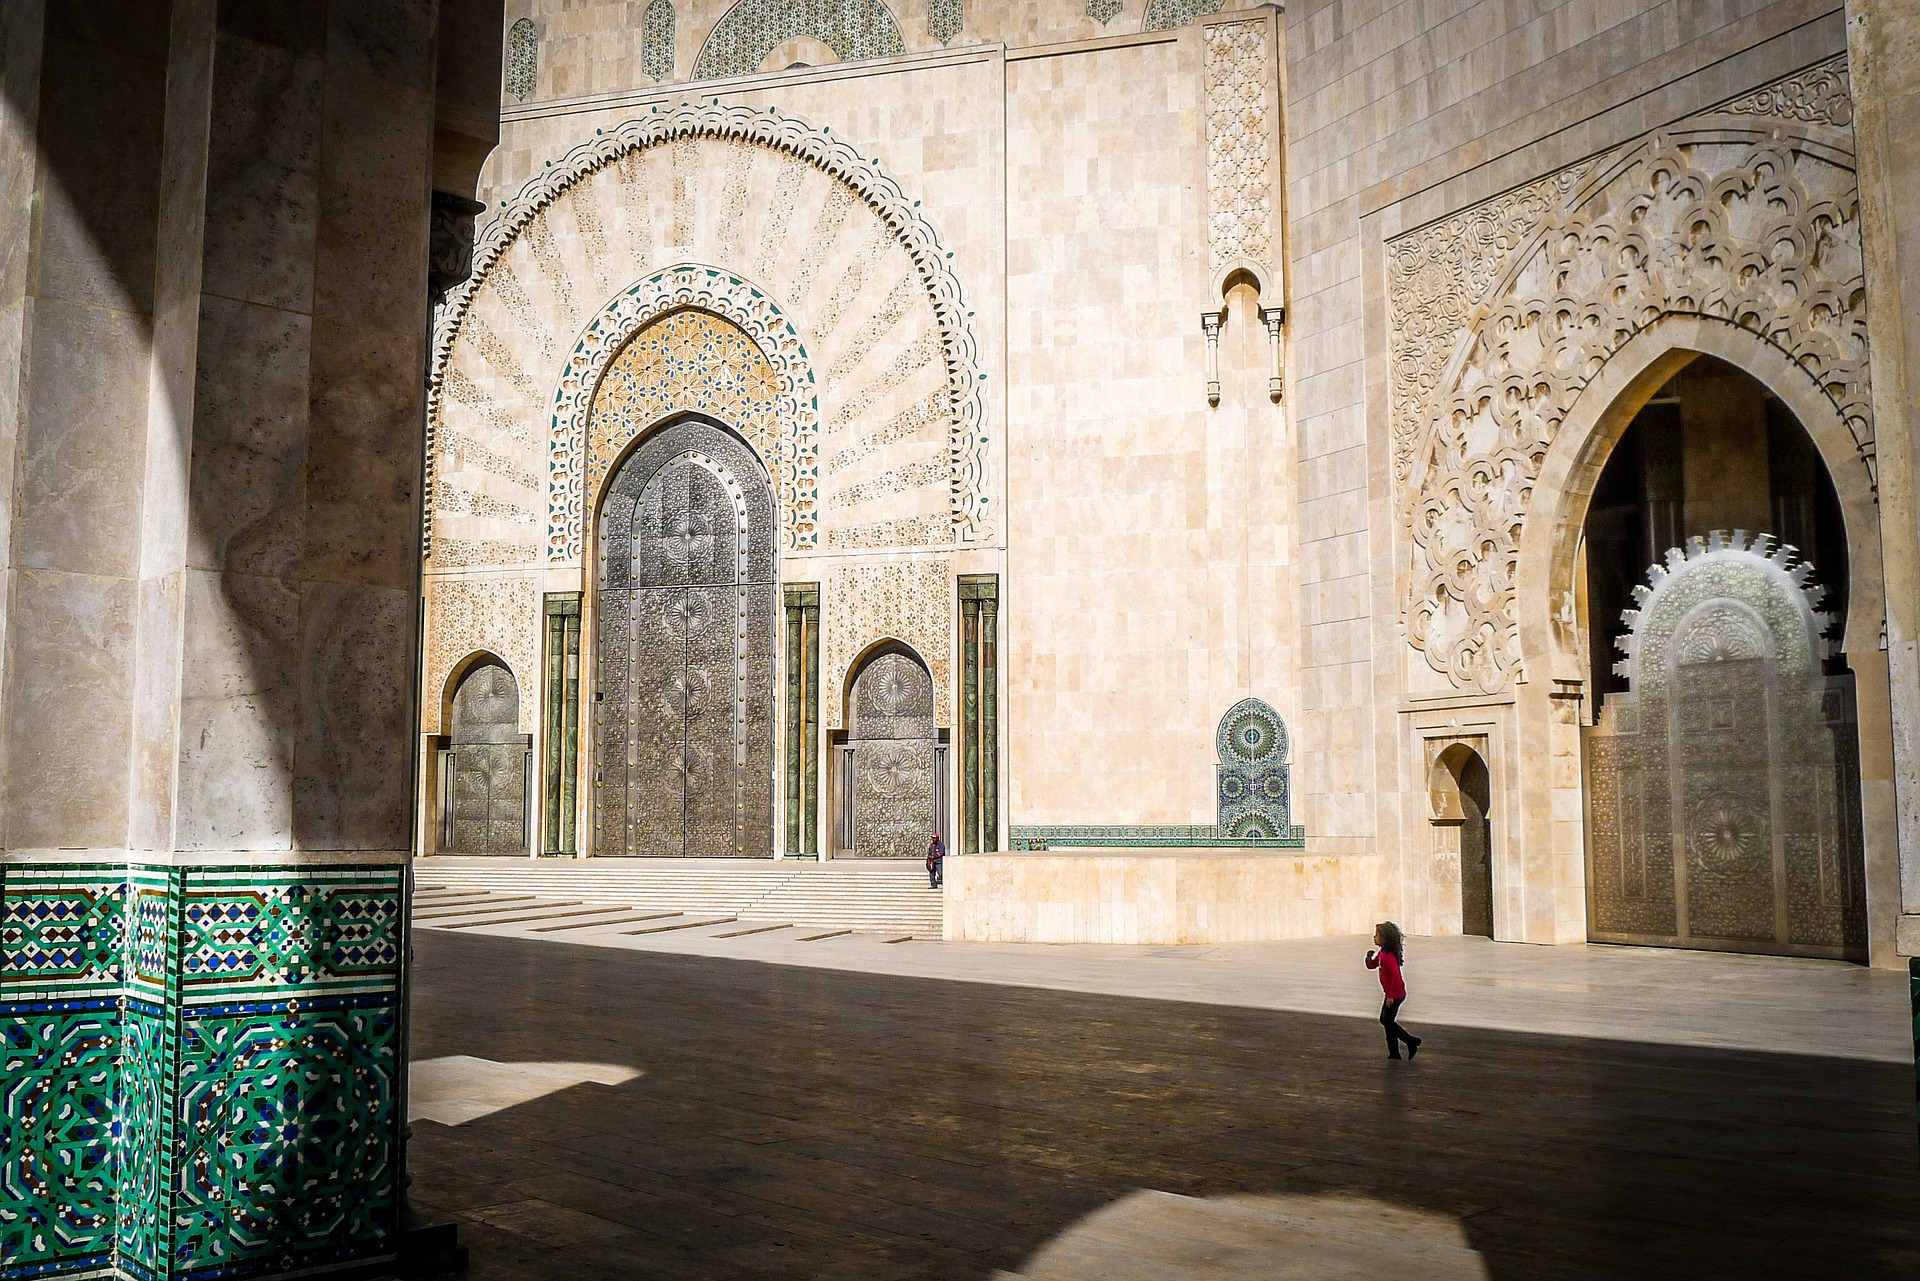
\includegraphics[width=0.5\columnwidth]
                                {contents/fig/mosque.jpg}
                \caption{caption示例}
            \end{figure}
        \end{texcodenoshad}
        \tcblower
        \begin{figure}[H]
            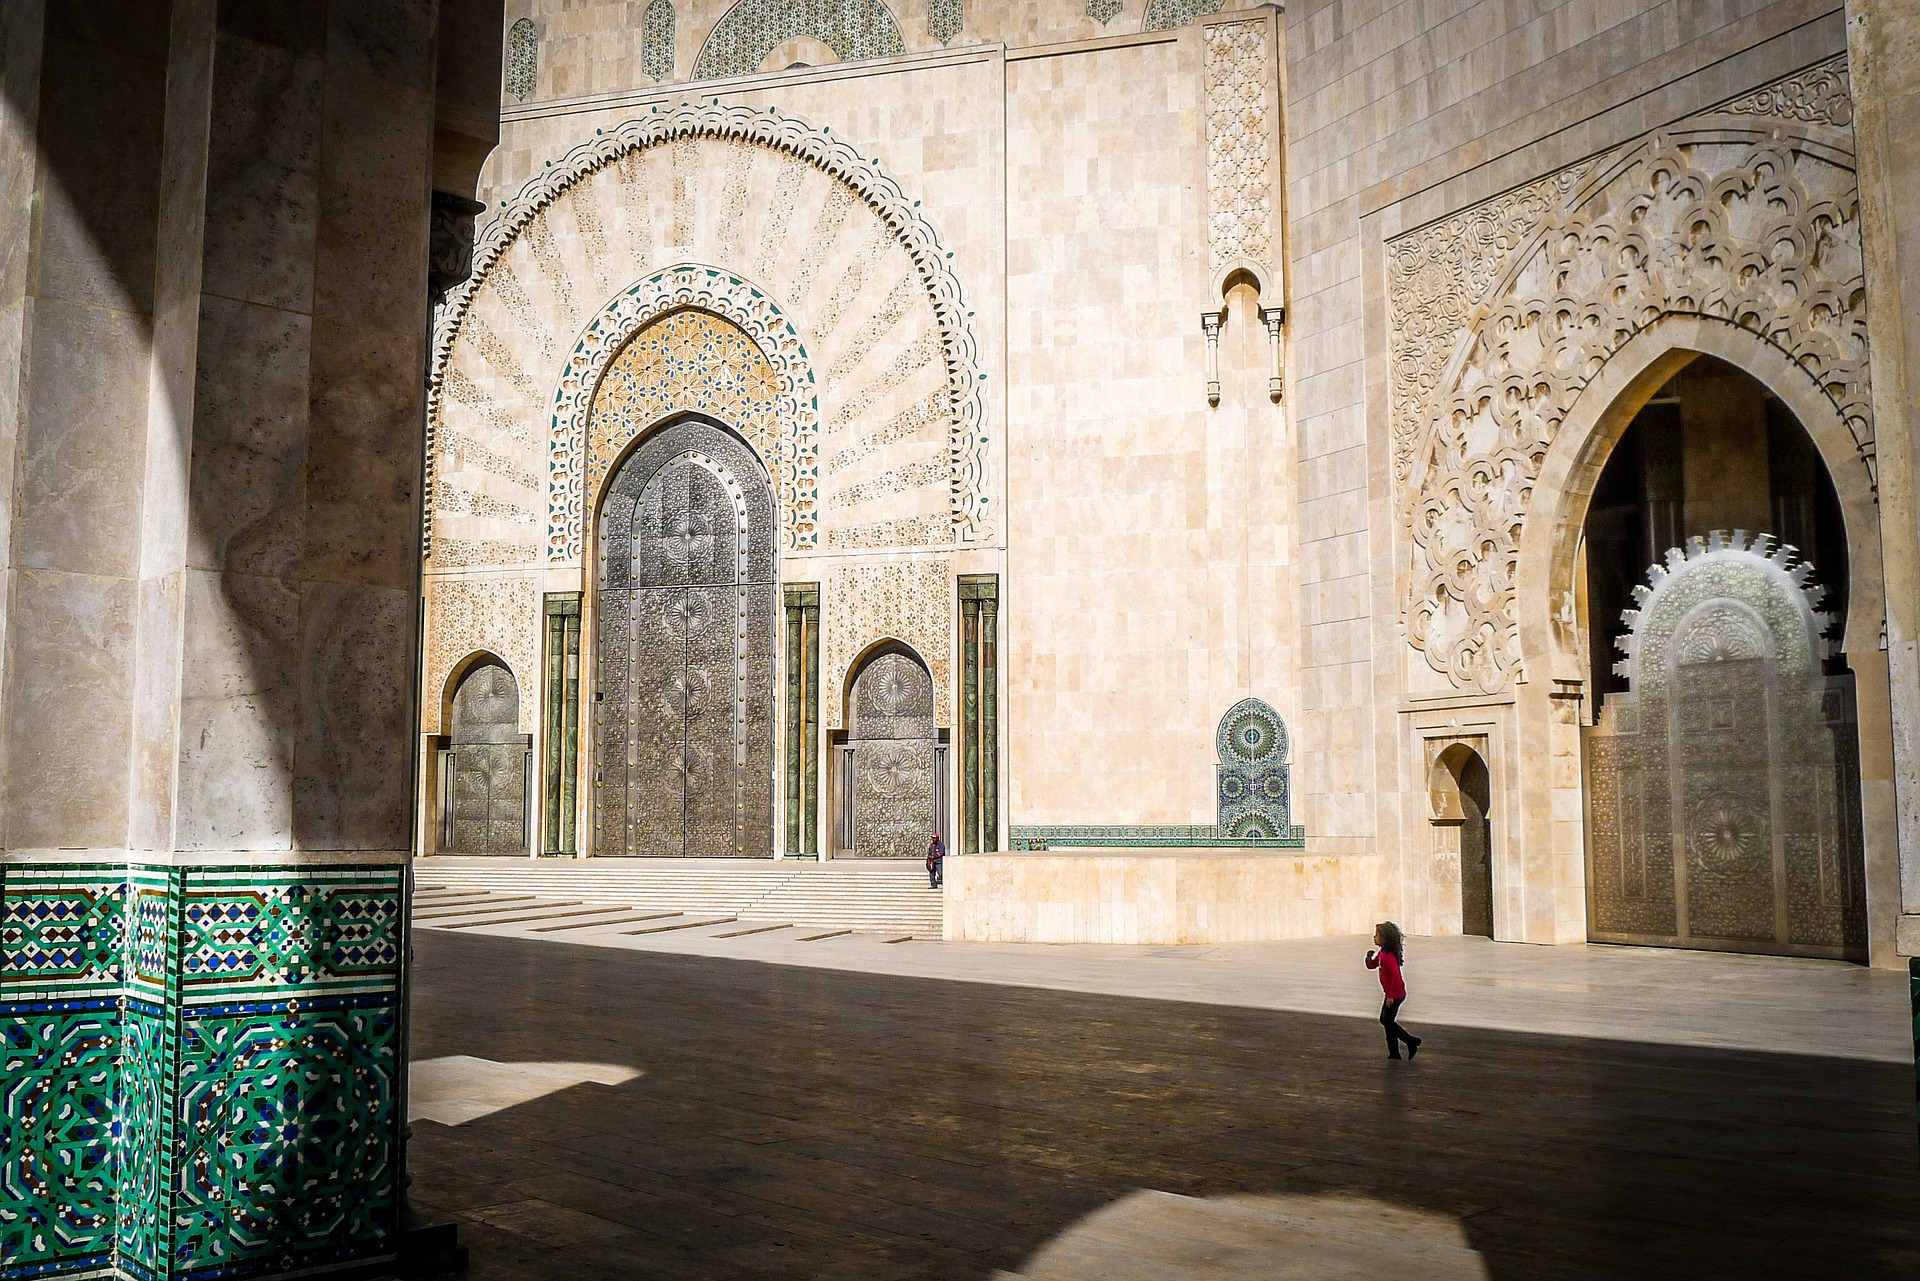
\includegraphics[width=0.5\columnwidth]
                            {contents/fig/mosque.jpg}
            \caption{caption示例}
        \end{figure}
    \end{texsepcode}
    如果要居中,则在Float环境中添加\highunderline{\textbackslash{}centering}即可(也可以在Float外或者Float内嵌套\highunderline{center}环境。)
    \begin{texsepcode}
        \begin{texcodenoshad}
            \begin{figure}[H]
                \centering
                \includegraphics[width=0.5\columnwidth]{contents/fig/mosque.jpg}
                \caption{居中示例}
            \end{figure}
        \end{texcodenoshad}
        \tcblower
        \begin{figure}[H]
            \centering
            \includegraphics[width=0.5\columnwidth]{contents/fig/mosque.jpg}
            \caption{居中示例}
        \end{figure}
    \end{texsepcode}
    \subsubsection{更改Float说明格式}
    默认中文下,\LaTeX{}会将表格编号为\textbf{表 n.},将图片编号为\textbf{图 n.},有时候我们可能有重新定制显示的需求,这实际上需要重新设置caption,具体如何设置请参考该宏包。

    % \todo{查看注释,又是个大的}
    % http://www.peteryu.ca/tutorials/publishing/latex_captions



    \subsection{Figure}\label{sub:figure}
    插入图片的基本使用可以参考\Ref{sec:graphics}一节,这里主要描述使用\highunderline{Figure}环境实现的各种图片的排版操作。

    \subsubsection{插入单张图片}
    在上一节已经有所演示,只需要用\highunderline{figure}环境包裹\highunderline{\textbackslash{}includegraphics}命令即可。
    
    \subsubsection{插入多个图片}
    插入多个图片可以直接在\highunderline{figure}环境中插入多个\highunderline{\textbackslash{}includegraphics}命令,但有时候需要对多个图片分别描述,因此需要使用\highunderline{subfigure}环境,如下:
    \begin{texshow}
        \begin{figure}[H]
            \subfigure[图片A]{ \label{subfig:show-a} % 标签永远都是可选项,需要引用的时候才需要添加
                \includegraphics[width=0.4\columnwidth]{mosque.jpg}
                \hspace{0.05\columnwidth} %声明水平间距,可以不添加,或者根据实际大小灵活更改
            }
            \subfigure[图片B]{
                \includegraphics[width=0.4\columnwidth]{mosque.jpg}
            }
            \caption{子图演示}
            \label{fig:sub-figure-show}
        \end{figure}
        % 如果需要居中,添加center环境或者使用\centering命令即可
    \end{texshow}
    
    % \todo{更改label/Tikz绘图/格式支持}
    % \subsubsection{插入环绕型图片}
    % \todo{环绕型图片}
    

    \subsubsection{列出图片目录}
    有时会有单独将所有的图片列出目录的需求,此时使用\highunderline{\textbackslash{}listoffigures}命令。
    
    \begin{quotation}
        一般是在文章目录后列出图片目录和表格目录。
    \end{quotation}
    
    % 如果需要手工插入图片目录,则使用
    
    
    \subsection{Table}\label{sub:table}
    
    \subsubsection{列出表格目录}
    有时会有单独将所有的表格列出目录的需求,此时使用\highunderline{\textbackslash{}listoftables}命令。
    
    \begin{quotation}
        一般是在文章目录后列出图片目录和表格目录。
    \end{quotation} %浮动窗口
    \section{注释与引用}\label{sec:注释与引用}
    \subsection{脚注}
    \subsubsection{基本使用}
    脚注使用\highunderline{\textbackslash{}footnote{内容}}命令:
    \begin{texshow}
        被脚注的文本\footnote{脚注内容}
    \end{texshow}
    \subsubsection{更改标记风格}
    需要重新定义\highunderline{\textbackslash{}thefootnote}来实现更改标记风格:

    \begin{texcode}
        被脚注的文本\footnote{脚注内容}\\
        \renewcommand{\thefootnote}{\roman{footnote}}
        被脚注的文本\footnote{脚注内容}
    \end{texcode}

    
    被脚注的文本\footnote{脚注内容}\\\renewcommand{\thefootnote}{\roman{footnote}}
    被脚注的文本\footnote{脚注内容}

    关于各种风格的数字显示方式,查看
    \subsubsection{重新计数脚注标记}
    如果只是要指定某个脚注的下标,可以直接通过添加参数的方式:
    \begin{texshow}
        被脚注的文本\footnote[12]{脚注内容}
    \end{texshow}


    脚注标记的计数也是用\LaTeX{}中的计数器来计数的,名字是\highunderline{footnote},因此要重新计数,只需要重置计数器\footnote{关于计数器,可以参考\Ref{subsub:counter}}即可:
    \begin{texcode}
        被脚注的文本\footnote{脚注内容}\\
        \setcounter{footnote}{5}
        被脚注的文本\footnote{脚注内容}
    \end{texcode}

    被脚注的文本\footnote{脚注内容}\\
        \setcounter{footnote}{5}
    被脚注的文本\footnote{脚注内容}

    \subsection{边注}

    \subsubsection{基本使用}
    边注是指在书两侧的注释,其在某种程度上比脚注更方便一些,因为边注直接显示在页面的一边\marginnote{就像这样。},读者不需要将视线移动太多就能看到相应的注释。

    最简单的边注,使用\highunderline{\textbackslash{}marginpar[left]\{right\}}命令。\marginpar{最简单的边注}如果是单侧布局(即不分奇偶页),那么边注仅显示在右侧,如果是双侧布局,则会显示在相应的外侧。如果是双栏布局,那么就会显示在靠近的一侧。

    \subsubsection{marginnote宏包}
    内置的这两种命令对于一些环境的支持不是很好,比如显示在公式的一侧,或者是显示在脚注的一侧,如果原生命令无法满足需求,那么就可以使用扩展宏包\highunderline{marginnote}。

    首先使用marginnote宏包后,\highunderline{geometry}就增加了可以控制边注大小和间隔的参数,如下:
    \begin{texcode}
        \usepackage[top=Bcm, bottom=Hcm, outer=Ccm, inner=Acm, 
            heightrounded, 
            marginparwidth=Ecm, marginparsep=Dcm]{geometry}
    \end{texcode}

    在设置好边距后,如果要添加边注,使用\highunderline{\textbackslash{}marginnote}命令:
    \begin{texshow}
        这里是一段难懂的命令\marginnote{这是一段解释的文字。}。
    \end{texshow}
    
    上面使用的命令如果更换为marginpar,在演示环境中会报错,这也是为什么推荐使用marginnote的原因。

    \subsection{标签}\label{sub:标签}
    \LaTeX{}支持在任意位置添加标签,从而可以很方便的建立链接,如\marginnote{从实现中可以看到标签的定义支持中文和一些标点,另外最好遵循某种规范,方便寻找}:
    \begin{texshow}
        如何实现一段标签可以查看该示例:\label{ex:标签示例}
    \end{texshow}
    要引用只需要使用内置命令\highunderline{\textbackslash{}ref}即可:
    \begin{texshow}
        如何使用引用可以参考\ref{ex:标签示例}节的介绍。
    \end{texshow}
    \begin{texshow}
        我们建议初学者浏览\pageref{sub:快速入门}页来查看如何入门\LaTeX{}
    \end{texshow}

    注意带有引用的位置均需要编译两次来完成,第一次编译只会形成问号,这是正常的。
    \subsubsection{其他的引用需求}
    ref命令只会显示相应位置的节号,而label命令实际上只是建立一种链接关系,因此,如果要更改引用部分的文字,我们可以使用\highunderline{hyperref}宏包中的\highunderline{\textbackslash{}hyperref}命令:
    \begin{texshow}
        % \usepackage{hyperref}
        这里有一个\hyperref[ex:标签示例]{标签示例}
    \end{texshow}
    注意如果链接到一个URL,那么使用的是\highunderline{\textbackslash{}href}命令,而且两者的参数填写方法也不一样:
    \begin{texshow}
        关于hyperref宏包的具体参数,可以参考其文档,或者查看
        \href{https://en.wikibooks.org/wiki/LaTeX/Hyperlinks}
        {Wiki-Hyperlinks}
    \end{texshow}

    另外,\highunderline{nameref}宏包提供了显示章节号的命令\highunderline{\textbackslash{}nameref}:
    \begin{texshow}
        % \usepackage{nameref}
        在\nameref{ex:标签示例}有一个示例
    \end{texshow}

    \subsection{参考文献}
    参考文献在\LaTeX{}中有多种管理方式,并且均可以被很方便的引用。\footnote{另外文献管理推荐使用\href{http://zotero.org}{zotero}}

    \subsubsection{直接引入}
    如果参考文献的数量比较少,不需要管理,那么可以直接使用\LaTeX{}的内置环境\highunderline{thebibliography},该环境会直接在相应位置生成参考文献列表:
    \begin{texshow}
        \begin{thebibliography}{9}
            \bibitem{lamport99}
              Leslie Lamport,
              \textit{\LaTeX: a document preparation system},
              Addison Wesley, Massachusetts,
              2nd edition,
              1994.
            \bibitem{SMOalgo}
                Platt,John C,
                \textit{Sequential Minimal Optimization: A Fast Algorithm for Training Support Vector Machines}
        \end{thebibliography}

        \begin{thebibliography}{1}
            \bibitem{tmc}
                Petersen,Pedersen,《The Matrix Cookbook》
        \end{thebibliography}
        
    \end{texshow}

    上述的代码中,环境后的参数为最大标签数(必填项),但是要注意的是,其中的参数不是数字大小,而是数字的位数,如果是一位数字,那么最大标签数是9;如果是两位,那么最大标签数是99(即使你所填的数字是59)。

    每一个参考文献,都用一个\highunderline{bibitem}来标识,\highunderline{bibitem}之后到下一个\highunderline{bibitem}之前的内容均属于该bibitem。

    如果要引用其中的其中的某一个参考文献,使用\highunderline{cite}命令\footnote{标签能够具有颜色和链接属性是因为hyperref库}:
    \begin{texshow}
        在这时候,有人发现了求解SVM的更快、更有效率的算法\cite{SMOalgo}
    \end{texshow}

    使用这种方法,跟目录等交叉引用项一样,需要用相应的编译器编译两次。

    \subsubsection{bibtex引入}

    直接引入虽然方便,但是当参考文献很多的时候,会很不方便,因为一般情况下,没有引用到的文献是不需要添加在参考文献中的,而且不同的组织,其参考文献如何排序都是有标准的,这些如果我们如果使用直接引入的方法,就必须全都考虑,就会很麻烦。由此,我们可以使用\highunderline{bibtex}来帮助我们管理参考文献和辅助引用。

    \highunderline{bibtex}基于\highunderline{.bib}文件,该文件可以被当做是数据库,可以把我们使用过的所有的参考文献都按照bibtex的格式放进去。其中,每一篇参考文献的格式均如下所示:
    \begin{texcode}
        @article{AbedonHymanThomas2003,
            author = "Abedon, S. T. and Hyman, P. and Thomas, C.",
            year = "2003",
            title = "Experimental examination of bacteriophage latent-period evolution as a response to bacterial availability",
            journal = "Applied and Environmental Microbiology",
            pages = "7499--7506",
            ...
        }
    \end{texcode}
    其中第一个参数是该引用的标识,而针对不同的引用(论文、期刊、书籍、网页...等),只需要按需填写不同的参数即可,如引用网页的示例格式如下:
    \begin{texcode}
        @misc{website:fermentas-lambda,
            author = "Fermentas Inc.",
            title = "Phage Lambda: description \& restriction map",
            month = "November",
            year = "2008",
            url = "http://www.fermentas.com/techinfo/nucleicacids/maplambda.htm"
        }
    \end{texcode}

    上述的内容可以全部存放到一个.bib文件中,也可以分门别类存放到多个.bib文件中,均可,只需要最后在使用的时候,在需要显式参考文献列表的位置添加如下的两行代码即可:
    \begin{texcode}
        \bibliographystyle{plain}
        \bibliography{bf1,bf2,...,bf3}
    \end{texcode}
    其中\highunderline{bibliographystyle}命令是表明参考文献展示的格式,包括排序方式,展示规范等,共有8种,分别为:
    \begin{center}
        % \newlength\tablewidth % if haven't define the length 'tablewidth'
        \setlength\tablewidth{\dimexpr (\textwidth -4\tabcolsep)}
        \begin{table}[H]
            \begin{tabular}{|p{0.3\tablewidth}<{\centering}|p{0.7\tablewidth}<{\centering}|}
                \hline
                plain&按字母的顺序排列,比较次序为作者、年度和标题.\\
                \hline
                unsrt&样式同plain,只是按照引用的先后排序.\\
                \hline
                alpha&用作者名首字母+年份后两位作标号,以字母顺序排序.\\
                \hline
                abbrv&类似plain,将月份全拼改为缩写,更显紧凑.\\
                \hline
                ieeetr&国际电气电子工程师协会期刊样式.\\
                \hline
                acm&美国计算机学会期刊样式.\\
                \hline
                siam&美国工业和应用数学学会期刊样式.\\
                \hline
                apalike&美国心理学学会期刊样式.\\
                \hline
            \end{tabular}
            \caption{参考文献的显示格式}
        \end{table}
    \end{center}

    第二行\highunderline{bibliography}命令表示在这里显示参考文献列表,参数填写参考文献都在哪些文件里,可多不可少。在具体编译完成后,相应位置只会显示文章中引用过的参考文献,.bib文件中其他的参考文献则不会显示。

    这种方式在文献的管理上确实比直接引用要好很多,但是也有一个非常麻烦的地方,那就是要用这种方式编译文件,需要编译四次,以使用xeLaTeX,编译main.tex为例,四次编译依次为:
    \begin{languagebox}[bash]
        xelatex main.tex
        bibtex main.aux
        xelatex main.tex
        xelatex main.tex
    \end{languagebox}
    注意第二次的参数是.aux文件而不是.tex文件,是在第一次编译后生成的,bibtex需要使用.aux文件来获取.tex文件中引用了哪些文献,从而生成相应的.bbl文件。.bbl文件的内容其实就是直接由bibtex从.bib文件中排好格式并且挑选出来相应文献后的\highunderline{thebibliography}环境,随后两次编译则是编译交叉引用的正常步骤。

    回头来看bibtex和.bib,它们实质上是依托于tex系统而形成的一套文献管理软件,其通过借助.tex文件编译后形成的引用信息来生成\LaTeX{}支持的参考文献环境。

 %脚注、边注、参考文献
    %! Author = saili
%! Date = 2019/8/25/0025

\section{颜色}\label{sec:color}
\subsection{引入}

如果想要更好的定义、使用和设置颜色,推荐使用%\highunderline[yellow]{xcolor}包
\begin{texcode}
\usepackage{xcolor}
\end{texcode}
xcolor包中定义了一些基本的颜色,有:

{\color{black}{black}},{\color{blue}{blue}}, {\color{brown}{brown}},{\color{cyan}{cyan}},{\color{darkgray}{darkgray}},{\color{gray}{gray}},{\color{green}{green}},{\color{lightgray}{lightgray}},{\color{lime}{lime}},{\color{magenta}{magenta}},{\color{olive}{olive}}

{\color{orange}{orange}},{\color{pink}{pink}},{\color{purple}{purple}},{\color{red}{red}},{\color{teal}{teal}},{\color{violet}{violet}},{\color{white}{white}},{\color{yellow}{yellow}}

另外xcolor中还定义了dvips中的68种标准色,如果要使用,需要在引入包时添加参数:
\begin{texcode}
\usepackage[dvipsnames]{xcolor}
\end{texcode}

\subsection{使用}
正如之前所使,几乎在任何一个可以更换颜色的地方,都可以更换相应位置的颜色。比如,{\color{red}{改变文字的颜色}}:
\begin{texshow}
{\color{red}这里放文字}\\
\textcolor{red}{这里放文字}%两者在设置文字颜色时等价
\end{texshow}

在大多数情况下,一些库或者自己生成的边框等,都可以通过设置其颜色属性或在外侧包裹color命令来实现变更颜色的方法。

\subsection{定义}
如果xcolor自带的颜色不足以使用,xcolor还提供了灵活的定义新颜色的方法,示例如下:

\begin{texcode}
\definecolor{light-gray}{gray}{0.95} %定义灰度
\definecolor{orange}{rgb}{1,0.5,0} %定义普通的rgb颜色(色值归一化为[0-1])
\definecolor{orange}{RGB}{255,127,0} %定义普通的rgb颜色(色值范围为0-255)
\definecolor{orange}{HTML}{FF7F00} %使用HTML设计时常用的方式,颜色由三个16进制数值组成
\definecolor{orange}{cmyk}{0,0.5,1,0} %使用印刷的色域,输入cmyk值
\end{texcode}

定义的颜色名字和xcolor自带的颜色名字具有相同的效果。

另外,在一些情况下,颜色还可以通过这样的一种语法来定义:
\begin{texcode}%默认底色是白色
    \colorlet{wblue}{blue!20} % 表示20%的蓝色+80%的白色
    \colorlet{bblue}{blue!20!black}% 表示20%的蓝色+80%的黑色
    \colorlet{bbg}{blue!20!black!30!green}% 表示20%的蓝色+30%的黑色+50%的绿色
\end{texcode}

在很多无法包裹color命令的情况下(如环境参数设置),大多是采用这种混合颜色(color mixes)的方式来设置颜色,如使用tcolorbox定义一个盒子:
\begin{texshow}
    \begin{tcolorbox}[colframe=blue!50!,colback=blue!20!]
        盒子内部
    \end{tcolorbox}
\end{texshow}

另外,如果要创建颜色的别名,也可以使用\highunderline{\textbackslash{}colorlet}:
\begin{texcode}
    \colorlet{mycolor}{someothercolor}
\end{texcode}

一般来说,新定义的颜色可以放到任何位置,但是为了规范,一般都倾向于将颜色统一定义在一个位置。

\subsection{其他环境下的颜色设置}

\subsubsection{表格}\label{sssec:color-table}
关于表格的颜色设置,参考\Ref{table-beauty}的说明

\subsection{超链接与引用}
超链接与引用的颜色,可以很方便的通过\highunderline[hlyellow]{hyperref}这个库来设置,只需要在导入库的时候定义参数即可,如:
\begin{texcode}
\usepackage[colorlinks,
linkcolor=black,
urlcolor=blue,
anchorcolor=blue,
citecolor=green]{hyperref}
\end{texcode}

\begin{texshow}
    \href{https://en.wikibooks.org/wiki/LaTeX/Hyperlinks}{Wiki-Hyperlinks}
\end{texshow}
关于设置的颜色对应哪个区域,以及更多的参数,可以参考\href{https://en.wikibooks.org/wiki/LaTeX/Hyperlinks}{Wiki-Hyperlinks}

\subsection{分割线}

\begin{texshow}
    %\rule[水平高度]{长度}{粗细}
    \color{red}{\rule[-10pt]{5cm}{0.05em}}
\end{texshow}

\subsection{颜色相关工具}
\subsubsection{LatexColor}
网站链接:\href{http://latexcolor.com/}{LatexColor}

点击看好的颜色直接复制定义颜色的语句,比较方便。
\begin{figure}[H]
    \centering
    \includegraphics[width=0.8\columnwidth]{\figpath{latexcolor.png}}
    \caption{latexcolor网站截图}
    \label{fig:latexcolor}
\end{figure}
 % 颜色
    
    \section{命令和环境}\label{sec:comm-envi}
    \LaTeX{}中除了正常的文字外,就只有命令和环境,一切均有命令和环境组成。甚至,环境也只是对命令的一种封装。完全可以将环境理解为互相联系的一组命令。
    \subsection{命令}
    \subsubsection{命令的基本使用}
    \LaTeX{}中大部分结构均为命令,调用命令的一般格式如下:
    \begin{texcode}
        \command[]{}{}..{}
    \end{texcode}
    其中command是命令名,使用反斜杠表示\footnote{所以如果要在\LaTeX{}中表示反斜杠需要使用\textbackslash{}textbackslash},\highunderline{[]}中的内容是可选项,一般省略,会被默认值替代,\highunderline{\{\}}中的内容是必选项,如果加大括号则为括号中的内容,否则则为命令后直到\highunderline{域边界\footnote{域边界根据不同的命令各有不同,这个我目前还没有查到相关的解释}}的内容。

    \begin{texshow}
        \textbf 粗体字
    \end{texshow}
    \subsubsection{命令的定义}
    如果要定义一个命令,使用\highunderline{\textbackslash{}newcommand}命令\footnote{该命令属于内置命令},如下:
    % 参考 https://en.wikibooks.org/wiki/LaTeX/Macros#New_environments
    
    \begin{texshow}
        \newcommand{\lmd}{$\lambda$\\}
        \lmd\lmd{}\lmd{Try it}
    \end{texshow}

    其中\highunderline{\textbackslash{}lmd}定义了一条名字为lmd的命令,第二个大括号中表示命令所代表的内容,在这里是一个符号加换行符。这种方式常用于代替某变量或符号,方便统一修改。注意不能够使用该命令定义一个已经存在的命令。\footnote{但可以\textbf{重新定义}该命令,参考\Ref{subsub:renewcomm}}

    如果要定义带有参数的变量,则需要添加参数选项:
    \begin{texshow}
        \newcommand{\myy}[1]{$y_{#1}$}
        \myy{1},\myy{2},\myy{3},\myy{n}
    \end{texshow}
    其中\highunderline{[1]}表示该命令可以有一个参数,\highunderline{\#{}1}表示参数放置的位置。

    \LaTeX{}命令最多支持九个参数,只需要更改参数数量,并在命令内容里添加相应的参数位置即可\footnote{注意,参数数量和具体不同参数的个数必须相同}
    
    \LaTeX{}还支持默认值,但只允许设置第一个参数有默认值,如下:
    \begin{texshow}
        \newcommand{\eqs}[3][2]{$(#3+#2)^#1,#1$\\}
        \eqs{a}{b}
        \eqs[5]{x}{y}
        \eqs{a}{b}{c}
    \end{texshow}
    其中\highunderline{[3]}表示该方法有三个参数,\highunderline{[2]}表示该方法第一个参数的默认值为2。注意上面的示例还演示了一个参数可以在不同的位置使用多次。

    对第三行命令调用的解释:该命令只选取了前两个作为参数,第三个由于大括号实际上是作为域的定界符,显示时会被忽略,因此实际上只代表了c这一个字符,按顺序显示在该命令后面。

    \subsubsection{命令的重新定义}\label{subsub:renewcomm}
    \LaTeX{}中最灵活的一点就是命令可以被重新定义,这使得我们可以更灵活的控制文档,但也因为这个原因,很多包之间对命令的复写会导致其相互冲突,如\highunderline{enumerate}宏包和\highunderline{enumitem}宏包。

    命令的重新定义和命令的定义方式几乎一样,只有两点不同:
    \begin{itemize}
        \item 使用\highunderline{\textbackslash{}renewcommand}命令
        \item 定义的命令必须是已经定义过的。
    \end{itemize}

    \subsection{环境}
    \subsubsection{环境的基本使用}
    环境的使用需要一对命令:\highunderline{\textbackslash{}begin}和\highunderline{\textbackslash{}end},如居中环境的使用:
    \begin{texshow}
        \begin{center}
            居中环境中的文字会居中。
        \end{center}
    \end{texshow}
    使用环境和使用命令非常相似,其一般格式如下:
    \begin{texcode}
        \begin{envi}[]{}{}..{}
            ...
        \end{envi}
    \end{texcode}
    \subsubsection{环境的定义}
    环境的定义使用\highunderline{\textbackslash{newenvironment}}命令,基本格式如下:
    \begin{texcode}
        \newenvironment{name}[num][default]{before}{after}
    \end{texcode}
    一个示例如下,从这个示例里可以看到环境之间可以互相嵌套:
    \begin{texshow}
        \newenvironment{titleenv}
        {
            \begin{center}居中标题\end{center}
        }
        {
            \\\rule{\textwidth}{1mm}
        }

        \begin{titleenv}
            正文内容
        \end{titleenv}
    \end{texshow}

    环境的参数使用方法和命令的参数使用方法完全一致,这里仅提供一个示例:
    \begin{texshow}
        \newenvironment{king}[2][Title Name]
        {
            \begin{center} \textbf{#1:#2}\\
        }
        {
            \end{center}
        }
        \begin{king}{参数二位置}
            这是多参数省略一参的一个示例
        \end{king}
        \begin{king}[参数一位置]{参数二位置}
            这是多参数的一个示例
        \end{king}
    \end{texshow}
    注意上面的示例中,参数只能放到\highunderline{before}区域,不能放到\highunderline{after}区域;另外可以通过在开始时添加一个环境头,结束时添加一个环境尾来实现一定的复杂逻辑。

    另外,\LaTeX{}中这种环境的定义是最为基本的定义,这种环境基本是可以随意嵌套的,但还有一些环境实际上更为复杂,也不是通过这种定义手段定义的,因此随意嵌套可能会出问题\footnote{具体的解释可以查看\href{https://www.zhihu.com/question/68657047/answer/266169094}{这篇回答}}
    

    \subsubsection{环境中的命令}
    在环境中可以定义命令,这样定义命令仅可以在环境中使用,如\highunderline{itemize}环境中的\highunderline{item}命令。
    
    定义方法没有其他的区别,仅在使用参数的时候,需要使用连续的两个\#{}来表示命令的参数\footnote{否则会报:\highunderline{! Illegal parameter number in definition of \textbackslash{}topics.}},一个示例如下:
    \begin{texshow}
        \newenvironment{topics}[1]
        {
            \newcommand{\topic}[2]{ \item{##1,##2} }
            Topics:#1
            \begin{itemize}
        }
        {\end{itemize}}
        \begin{topics}{标题}
            \topic{参数一}{参数二}
            \topic{参数一}{参数二}
        \end{topics}
        % \eitem{a}{b} 环境外使用会报错误:Undefined control sequence.
    \end{texshow}

    \subsubsection{环境的重新定义}
    环境的重新定义参考命令的重新定义和环境的定义方法,基本完全相同:

    \newenvironment{titleenv}{\begin{center}居中标题\end{center}}{\\\rule{\textwidth}{1mm}}
    \begin{texshow}
        \renewenvironment{titleenv}[1][居中标题]{
            \begin{center}#1\end{center}
        }{\\\rule{\textwidth}{1mm}}
        
        \begin{titleenv}[我的标题]
            正文环境
        \end{titleenv}
    \end{texshow}

    \subsection{高级命令与环境}
    部份宏包使用了更底层的机制,使得它们可以完成和一般形式不同的命令和环境定制,如对参数名的支持:
    \begin{texshow}
        \begin{tcolorbox}[colframe=blue!50!,colback=blue!20!]
            盒子内部
        \end{tcolorbox}
    \end{texshow}
    如果要实现这种效果,可以去学习底层的TeX命令,也可以使用宏包\highunderline{xkeyval}来完成\footnote{虽然该宏包的使用也和一般语法不同},精力有限不多介绍,留坑以后填。

    \subsection{计数器}\label{subsub:counter}

    \subsubsection{基本介绍}
    \LaTeX{}内置的计数器有23个,其中17个为序号计数器,6个为控制计数器(只是用途不同,本质都是计数器的一种)。

    \begin{center}
        % \newlength\tablewidth % if haven't define the length 'tablewidth'
        \setlength\tablewidth{\dimexpr (\textwidth -8\tabcolsep)}
        \begin{table}[H]
            \begin{tabular}{|p{0.24\tablewidth}<{\centering}|p{0.23\tablewidth}<{\centering}|p{0.26\tablewidth}<{\centering}|p{0.26\tablewidth}<{\centering}|}
                \hline
                计数器名&用途&计数器名&用途\\
                \hline
                part&部序号计数器&equation&公式序号计数器\\
                \hline
                chapter&章序号计数器&page&页码计数器\\
                \hline
                section&节序号计数器&footnote&脚注序号计数器\\
                \hline
                subsection&小节序号计数器&mpfootnote&小页环境中的脚注序号计数器\\
                \hline
                subsubsection&小小节序号计数器&enumi&排序列表第1层序号计数器\\
                \hline
                paragraph&段序号计数器&enumii&排序列表第2层序号计数器\\
                \hline
                subparagraph&小段序号计数器&enumiii&排序列表第3层序号计数器\\
                \hline
                figure&插图序号计数器&enumiv&排序列表第4层序号计数器\\
                \hline
                table&表格序号计数器& &\\
                \hline
            \end{tabular}
            \caption{\LaTeX{}内置的序号计数器}
        \end{table}
    \end{center}


    % 参考 https://blog.csdn.net/archielau/article/details/7976507
    % http://softlab.sdut.edu.cn/blog/subaochen/2017/07/latex%E7%9A%84%E8%AE%A1%E6%95%B0%E5%99%A8%EF%BC%88counter%EF%BC%89/

    \begin{center}
        % \newlength\tablewidth % if haven't define the length 'tablewidth'
        \setlength\tablewidth{\dimexpr (\textwidth -4\tabcolsep)}
        \begin{table}[H]
            \begin{tabular}{|p{0.20\tablewidth}<{\centering}|p{0.80\tablewidth}<{\centering}|}
                \hline
                bottomnumber&控制每页底部可以放置浮动体的最大数量,默认值为1\\
                \hline
                dbltopnumber&双栏排版时,控制每页顶部可放置跨栏浮动体的最大数量,默认值为2.\\
                \hline
                secnumdepth&控制层次标题的排序深度,book和report默认为2,article默认为3\\
                \hline
                topnumber&控制每页顶部可放置浮动体的最大数量,默认为2\\
                \hline
                totalnumber&控制每页中可放置浮动体的最大数量,默认值为4\\
                \hline
                tocdepth&控制章节目录的目录深度,文类book和report默认值为2,而article默认值为3,。通常secnumdepth≥tocdepth\\
                \hline
            \end{tabular}
            \caption{\LaTeX{}内置的控制计数器}
        \end{table}
    \end{center}

    \subsubsection{生成计数器}
    新建一个计数器:
    \begin{texcode}
        \newcounter{NameOfTheNewCounter}
    \end{texcode}
    如果在新建时,需要你的计数器在其他计数器增加的时候被清零,可以通过额外添加计数器参数的方式来实现:
    \begin{texcode}
        \newcounter{NameOfTheNewCounter}[NameOfTheOtherCounter]
    \end{texcode}
    对一个已存在的计数器,如果需要它在某个其他计数器增加的时候被清零,可以通过以下的命令:
    \begin{texcode}
        \counterwithin*{NameOfTheCounter}{NameOfTheOtherCounter}
    \end{texcode}
    
    为某个计数器加1:
    \begin{texcode}
        \stepcounter{equationschapter}
    \end{texcode}
    指定该计数器的值:
    \begin{texcode}
        \setcounter{NameOfTheNewCounter}{number}
    \end{texcode}
    为某个计数器增加任意数值(该数值可以是负数),可以使用以下命令:
    \begin{texcode}
        \addtocounter{NameOfTheNewCounter}{number}
    \end{texcode}

    如果要获取某个计数器的值(上述的命令有的参数需要传入number而不是某个counter),那么使用以下的命令来返回一个number:
    \begin{texcode}
        \value{NameOfTheNewCounter}
    \end{texcode}
    
    \subsubsection{计数器风格}
    请参考\Ref{subsub:number}

    \section{代码环境方案}
    \subsection{程序代码}
    \subsubsection{抄录环境}
    \subsubsection{listing}
    \subsubsection{minted}
    \subsubsection{最佳实践:tcolorbox}
    \subsection{伪代码}
    
    % https://blog.csdn.net/simple_the_best/article/details/52710794 伪代码环境
    \subsection{树结构}
    % Latex树状结构-Forest http://softlab.sdut.edu.cn/blog/xuqianhui/2017/06/28/latex%e6%a0%91%e7%8a%b6%e7%bb%93%e6%9e%84-forest/
    \section{编写结构}
    
    \todo{引入文件/引用问题/编译参数/目录/目录问题/代码风格/abspath}
    
    \todo{更改目录结构后,对各种库、bibtex的影响和解决}

    \section{库使用}
    \subsection{minipage}\label{sub:minipage}
    minipage宏包用于在一页中创建一个小的页面(实质是一个盒子),也具有很强的可定制性。
    \subsection{tcolorbox}
    本手册使用的全部带颜色的边框均为tcolorbox的实现,其基本的使用非常简单,在熟悉\LaTeX{}的基本操作后,可以查看tcolorbox的宏包说明手册来完成,其所有的边框,间隔,圆角,文字,分割线都可以自定义,同时还对代码的显示进行了封装,可以更自由的定制代码的显示风格。

    \subsection{adjustbox}
    是一个用于任意调整“盒子”位置的宏包,盒子是\LaTeX{}中的基本单位,所以该宏包在一些场合的定制性非常的强。
    
    \section{高级使用}
    \todo{有生之年系列:文档类撰写、Latex语言深入、库撰写、Tex编译结构}
    \todo{MakeFile编写}

    \section{模板收录}
    国赛模板:\href{https://github.com/latexstudio/CUMCMThesis}{Github链接}
    
    \todo{简历模板、PPT模板、笔记模板、书模板...}


\end{document}
% 
